\documentclass[journal]{IEEEtran}

\usepackage{tikz}
\usepackage{colortbl}
\usepackage{amsthm} 
\usepackage{amsmath}
\usepackage{url}
\usepackage[linesnumbered,algoruled,boxed,lined]{algorithm2e}


% for styling tables
\makeatletter
    \def\CT@@do@color{%
      \global\let\CT@do@color\relax
            \@tempdima\wd\z@
            \advance\@tempdima\@tempdimb
            \advance\@tempdima\@tempdimc
    \advance\@tempdimb\tabcolsep
    \advance\@tempdimc\tabcolsep
    \advance\@tempdima2\tabcolsep
            \kern-\@tempdimb
            \leaders\vrule
    %^^A                     \@height\p@\@depth\p@
                    \hskip\@tempdima\@plus  1fill
            \kern-\@tempdimc
            \hskip-\wd\z@ \@plus -1fill }
    \makeatother
    

\usepackage{listings}
\lstset{ %
language=java,                % choose the language of the code
numberstyle=\tiny,      % the size of the fonts that are used for the line-numbers
frame=Ltbr,
rulesep=.4pt,
mathescape, % Allows escaping to (La)TeX mode within $$,
stringstyle=\color{redb},
keywords=[1]{elseif, return, else, int, wire, bool, if, Boolean, do-together, foreach, endfor, endif, while, to, Let},
keywords=[2]{decl-list, init-list,next-list, wiredef-list, var-st, loc-st, append, assignment},
showstringspaces = false,
escapeinside={/*@}{@*/},
basicstyle=\small\ttfamily,
keywordstyle=[2]\color{darkred}\bf,
keywordstyle=[1]\color{blue}\bf,
commentstyle=\color{green},
alsoletter={-},
captionpos=b, %
breaklines=true
}


\newcommand{\edited}[1]{{\color{black} #1}}
\newcommand{\secondedited}[1]{{\color{black} #1}}
\newcommand{\thirdedited}[1]{{\color{black} #1}}

\newtheorem{theorem}{Theorem}
\newtheorem{proposition}{Proposition}





\hyphenation{op-tical net-works semi-conduc-tor}


\begin{document}


\title{Spatiotemporal contingency analysis for the Lebanese power grid using Apache Spark}


\author{Fatima K. Abu Salem$^{2}$, \and
Mohamad  Jaber$^{2}$, \and 
Chadi Abdallah$^{1}$, \and 
Omar Mehio$^{2}$, \and and Sara Najem$^{1}$
\thanks{$^1$ National Center for Remote Sensing, National Council for Scientific Research (CNRS), Riad al Soloh, 1107 2260, Beirut, Lebanon. Email: \texttt{\{snajem, chadi\}@cnrs.edu.lb}.}
\thanks{$^2$ Computer Science Department, American University of Beirut, Beirut, Lebanon. Email: \texttt{\{fa07, mj54, okm02\}@aub.edu.lb}.}
\thanks{Equally contributing author. Corresponding author: Sara Najem.}
}



% \texttt{\{fa07, mj54, okm02\}@aub.edu.lb}


% The paper headers
\markboth{IEEE Trans. of Computational Social Systems - SI: \emph{Parallel and Distributed Processing for Computational Social Systems}}%
{}


% make the title area
\maketitle
\begin{abstract}
We address a topological vulnerability analysis of the Lebanese power grid subject to random and cascading failures. Using an Apache Spark implementation that maps the topology of the grid to a complex network, we begin by developing a local structural understanding of the Lebanese power grid that reveals a certain level of decentralisation via numerous connected components. Our Apache Spark implementation simulates random and cascading sequences of events by which energy centers in Lebanon can be exposed and are at risk. The implementation is based on the bulk-synchronous parallel (BSP) model and maintains optimal work, linear communication time, and a constant number of synchronisation barriers. We complement our work with a spatial understanding of the exposed hotspots. Our results reveal that failures in the power grid are spatially long-range correlated, and that correlations decay with distance. In a couple of attack scenarios our Spark implementation achieves significant speedup on $16$ cores for a graph with about $9\times 10^5$ nodes. Scalability towards $32$ nodes improves when experimenting with replicas of the power grid graph that are double and quadruple the original size. This renders our work suitable to larger networks at many vital levels beyond the power grid.
\end{abstract}


\begin{IEEEkeywords}
Spatiotemporal, Spark, Power Grid, Parallel Computing, Graph
\end{IEEEkeywords}


\IEEEpeerreviewmaketitle

\maketitle

\section{Introduction}
\label{introduction}

In scale-free networks (SF) the probability of a node being connected to $k$ others exhibits a power-law distribution $P(k) \propto k^{-\alpha}$, which is a topological property affecting and controlling their resilience or the measure of their functionality subject to disruptions \cite{Newman:2003da,Gao:2015fg,Bashan:2013cja,2000Natur.406..378A}. Examples of this class of SF are the Internet, power systems, and transportations networks, which are real-world networks shown to be robust when subject to random failures, yet, displaying a high vulnerability when subjected to cascading ones \cite{Bompard:2011cd,DuenasOsorio:2009ff,2016arXiv160904310M,Cohen:2001hf}. 

In power systems, and unlike random failures which emerge locally, blackouts are severe events  associated with cascading behavior leading to global network collapse \cite{RosasCasals:2007td,Bompard:2009ga,Brummitt:2013jj,Daqing:2014bp,Albert:2004bw,Wang:2011js,Sole:2008cv}. Examples such as the one affecting the north-east in the US and eastern Canada in 2003 burdened the respective economies with ten billion dollars of direct costs \cite{Daqing:2014bp}. Such failures can be linked to either structural dependencies, where the damage spreads via structurally dependent connections, or functional overloads, where the flow goes through alternative paths leading to overloaded nodes. Thus, understanding the propagation of these failures becomes pivotal in developing and deploying protective and mitigating strategies. 

Large power systems and real-world networks in general exhibit an exponentially increasing combinatorial number of failure nodes. Older works tackling contingency analysis relied on approximate power flow solutions, exhibiting only a simplified analysis of all combinatorial contingencies \cite{EjebeAl79,Ekwue91}. These approaches also levy an overwhelming computational burden that cannot be accomplished in real-time. Also, traditional approaches that employ the $N$-1 criterion are only able to investigate the ability of the transmission system to lose a power line or a power generator without causing an overload failure elsewhere. Examples of such approaches are employed by the North American Electric Reliability Corporation (NERC) \cite{JinAl10}, and obviously do not capture the overload failures that propagate through interactions among a system's physical components. It thus becomes necessary to be able to perform $N$-$x$ ($x \geq2$) contingency analysis to assess whether a system can withstand the failure of any two or more components. In several leading works such as \cite{2000Natur.406..378A,JinAl10, DaqingAl14}, the power grid, particularly the network of its transmission lines, is analyzed using graph algorithms such as betweenness centrality and shortest paths. In this paper, we build on the approach in  \cite{2000Natur.406..378A} using an Apache Spark implementation of topological vulnerability analysis of the Lebanese power grid subject to random  and cascading failures. Beyond the scholarly aspects of our proposed work, our analysis contributes towards precision-based policy making and disaster response in a region marred by wars and under-development. 
 
Using elements from distributed algorithm design as well as spatial analysis, our work extends the approach of \cite{2000Natur.406..378A} in analysing the vulnerability of transmission lines to the assessment of that of the whole Lebanese power grid, including its generation, distribution, and transmission lines. However, in contrast to this cited body of work, our approach yields a system that is fault-tolerant to hardware failures and ensures locality of reference to avoid data movement. The choice of Spark also renders our system to be suitable for clusters of commodity computers with relatively slow and cheap interconnects, and susceptible to many machine failures. Our implementation is based on the BSP model and maintains optimal work, linear communication time, and a constant number of synchronisation barriers. 
%By targeted attacks, we do not merely allude to acts of aggression on power generating centers, but also to increasing consumption associated with a diminished national carrying capacity following the refugees influx.

Our manuscript is organized as follows. In Sec. \ref{background}, we present an overview of related work that tackles power grid resilience analysis as well as implementations of it that runs on distributed systems, and we describe some intrinsics related to Apache spark for big data distributed processing. In Sec. \ref{methods}, we present our distributed graph algorithm that builds on the loosely centralized structure of the Lebanese power grid using Breadth First Search and Vertex Betweenness Centrality, orchestrated using four scenarios known in the literature \cite{2000Natur.406..378A}. Each of these scenarios simulates a unique temporal mode of removal of vertices. In Sec. \ref{results}, we perform run-time analysis of our algorithm and obtain excellent scalability for some scenarios as the number of processing cores increases up to 16, a result which we attribute to the large number of connected components found in the Lebanese power grid and the fact that majority of connected components have a relatively small cardinality. In fact, scalability towards $32$ nodes improves when experimenting with replicas of the power grid graph that are double and quadruple the original size. We demonstrate the loss in connectivity in the power grid associated with each scenario, and obtain that the Lebanese power grid exhibits a relatively strong resilience thanks to its decentralised structure. We also perform a spatial correlation analysis of failures using the geocoding of vertices that lead to $90\%$ loss in connectivity. Our results reveal that failures in the power grid are spatially long-range correlated, and that correlations decay with distance. In Sec. \ref{conclusion}, we conclude with remarks around the impact of our work.%, particularly, as it relates to directing policy making. should current trends of refugee influx continue. It is our hope that our work can help answer questions such as: what factors will affect future observations at different locations on Lebanese soil? and what can be done to better manage our dwindling vital systems?  






\input{background}

\section{Materials and Methods}
\label{methods}

\subsection{Input Graph}

We build the network model using data provided by the Lebanese Ministry of Energy and Water. This dataset contains information about every power plant generator (sources for power), high-to medium voltage transmission substations, medium to low voltage distribution stations that disseminate power directly to subscribers, as well as transmission lines through which power dissipates. Transmission lines exist between generators and transmission substations, as well as among transmission substations, distribution substations, and finally, between transmission and distribution substations. 


\secondedited{
The power grid consists of generating stations responsible for the power production, which is transmitted through high voltage lines to demand centers, which then, in turn, distribute power to the consumers.  This design entails the emergence of a large number of connected components which is a universal feature of grids with a characteristic power-law degree distribution~\cite{RosasCasals:2007td,Bompard:2009ga,Brummitt:2013jj,Daqing:2014bp,Albert:2004bw,Wang:2011js,Sole:2008cv}.}
%
There are five major power plants in Lebanon. Transmission and distribution substations are such that they receive power from all of the major power plants, and so, if all but one such plant is hit, the entire network can still receive power. Because of this redundancy, the only way to achieve total failure is through the obvious choice of attacking all five power plants. 
%
\edited{
To exclude this obvious scenario from our contingency analysis, the data received directly from the Lebanese Ministry of Energy and Water does not include all five power plants from the associated graph model. This renders our contingency analysis completely focused on the irredundant nodes constituting transmission and distribution substations, where the corresponding graph representation of the power grid consists of several connected components. }
%
\secondedited{
We should note that in the original dataset these five vertices were assigned a tag directly by the Ministry of Energy and Water, which described them as redundant. Therefore no extra computational work was done to identify them. In the event that the power network fails to manifest a large number of connected components that permit for the kind of distribution we are adopting in the present manuscript, one can attempt to distribute/parallelise the low-level graph Betweenness Centrality and Single Source Shortest Paths algorithms employed, using, for example, a number of distributed and parallel tools available in~\cite{Bertolucci16,Djidev14,Edmonds10,Jin10,Kumbhare14,Redekopp13,Solomonik13}, to cite a few.}
%
Our analysis simulates attacks on both transmission as well as distribution substations. It also pursues inter-dependencies as failures propagate within a single connected component, and addresses the overall loss of connectivity to all subscribers as a result. Finally, our analysis adopts the idealised (and simplified) view that capacity across the transmission lines is never jeopardised, and thus failure of the network is a result of attacks on substations only.

\thirdedited{
Our resulting network model consists of an undirected, unweighted graph\footnote{Please note that this bears no impact on the performance if the graph is directed. First off, all of the algorithms used (e.g. strongly connected component and betweenness centrality) have variants that can tackle directed graphs. Moreover, these variants have the same work complexity as those for the undirected graph.} with $679965$ edges, representing transmission/distribution lines, and $899162$ vertices, representing transmission/distribution substations. This is one order of magnitude larger than the graph treated in \cite{2000Natur.406..378A}, and is a consequence of the fact that the given Lebanese power grid representation captures extremely fine grained spatial coordinates, yielding all distribution substations no matter how minor. Our distribution analysis of the degrees of vertices confirms that indeed, the resulting graph exhibits a power law distribution (Fig. \ref{fig:degree-vertices}).}
%Also, our analysis is holistic in the sense that it simulates attacks on both transmission as well as distribution substations. 
%insert figure here

\begin{figure}[!tbp]
  \centering
     {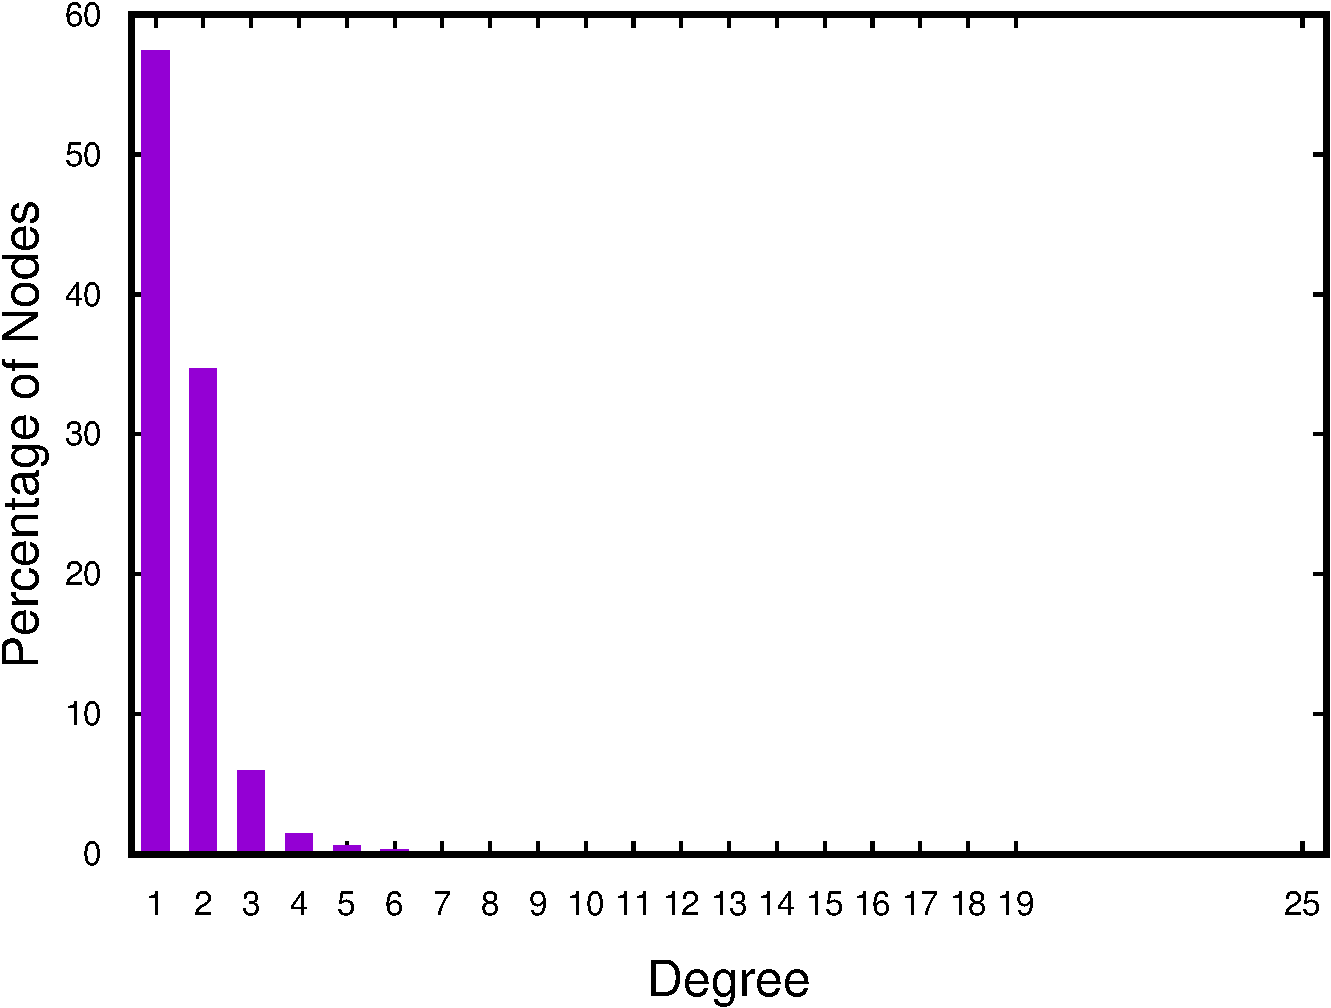
\includegraphics[scale=0.35]{bench/generated/degree-counter-crop.pdf}}
  \caption{Degree of vertices}
    \label{fig:degree-vertices}
\end{figure}

\begin{figure}
\centering
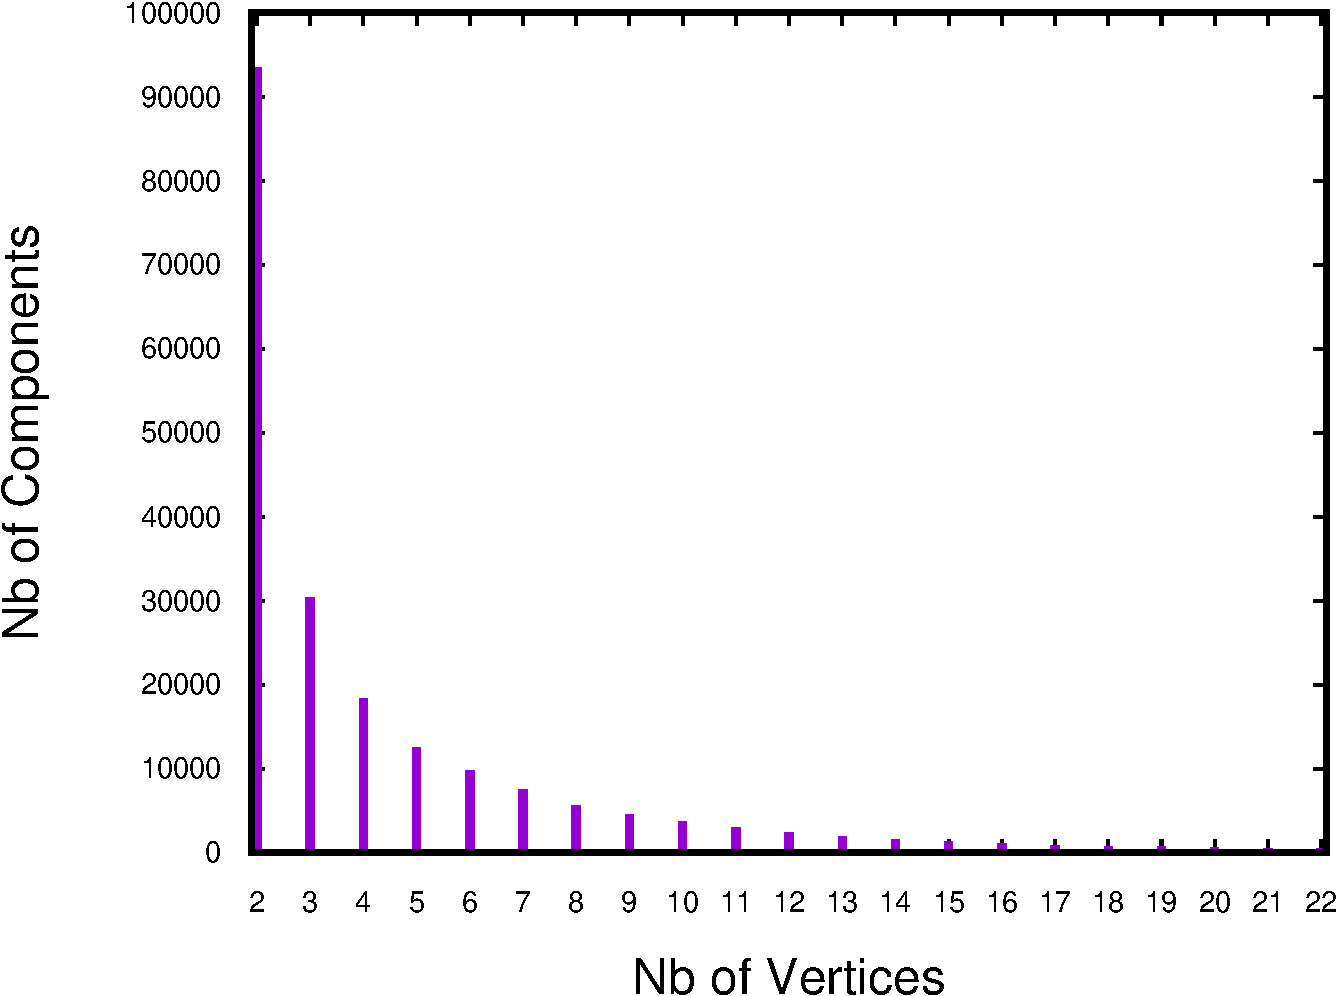
\includegraphics[scale=0.35]{bench/generated/frequency20-crop.pdf}
\caption{Distribution of components w.r.t. the number vertices (range from $2$ to $20$ vertices per component)}
\label{fig:vertices-components-20}
\end{figure}

\begin{figure}
\centering
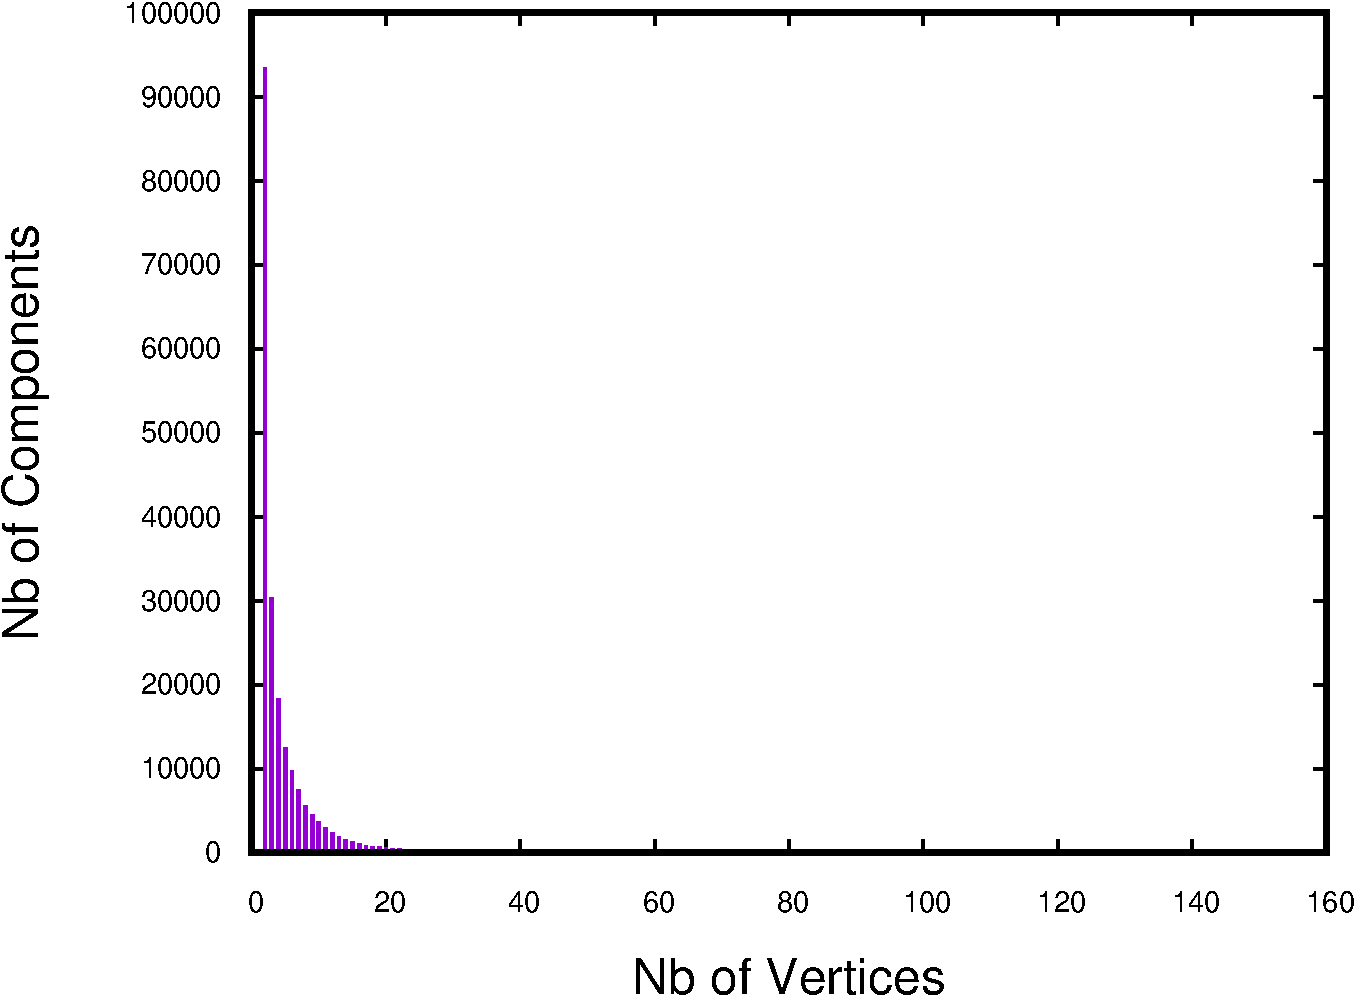
\includegraphics[scale=0.35]{bench/generated/frequencyall-crop.pdf}
\caption{Distribution of components w.r.t. the number vertices}
\label{fig:vertices-components-all}
\end{figure}

\begin{figure}
\centering
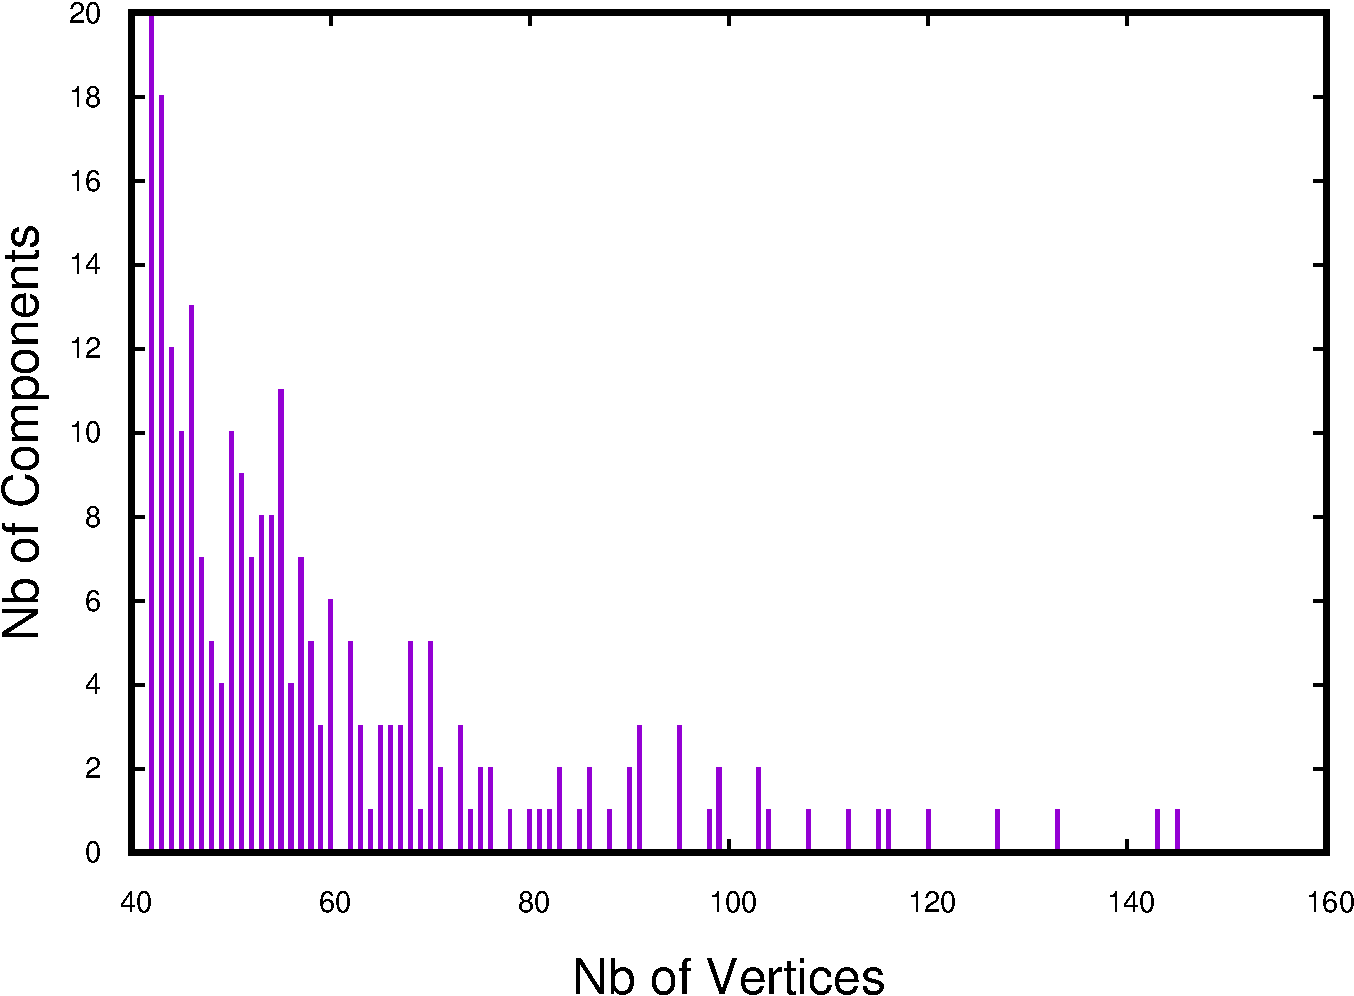
\includegraphics[scale=0.35]{bench/generated/frequency-selected-crop.pdf}
\caption{Distribution of components w.r.t. the number vertices (range from 40 to 140 vertices per component)}
\label{fig:vertices-components-40}
\end{figure}


% Because of this redundancy, the only way to achieve total failure is through the obvious choice of attacking all ten power plants. To exclude this obvious scenario from our contingency analysis, we remove all ten power plants from the associated graph model. This renders our contingency analysis completely focused on the irredundant nodes of the power grid. What remains are the high to medium step down stations that transform high voltage to medium voltage nodes as follows. As treated in \cite{2000Natur.406..378A}, a distribution substation is one that receives power from a single, high voltage transmission line, and distributes this on smaller voltage to consumers. However, when modeling the power grid here, we make no distinction between nodes representing transmission substations versus distributing substations. Since our distributed algorithm is aimed for big graphs, an exhaustive analysis of the power grid should be attempted, and as such, we preserve the power grid almost in its entirety with a few exceptions. 

\subsection{Random and Cascading Contingency Analysis}

Our baseline approach for navigating through node attacks follows that of \cite{2000Natur.406..378A}. A high level representation of the algorithm for implementing the random and cascading attacks is depicted in Algorithm~\ref{algo:random-cascading}. It captures both notions of node attack, followed by an evaluation of the loss in power flow capacity across the entire network.
%\begin{lstlisting}[language=java]
%attackGraph(Graph graph) {
%   for(i = 0 until |V|) {
%      select victim vertex v
%      remove vertex v
%      update loss with respect to v
%   }
%}
%\end{lstlisting}
%
\begin{algorithm}[ht]
\KwIn{Graph graph = (V, E)}
\KwOut{random and cascading attacks of the input graph}
    \SetKwFunction{FMain}{attackGraph}
    \SetKwProg{Fn}{Function}{:}{}
    \Fn{\FMain{graph}}{
        \For{$i \gets 0$ \KwTo $|V|$}
        {
        select victim vertex v\;
        remove vertex v\;
        update loss with respect to v\;
        }
}
\textbf{End Function}
 \caption{\edited{Random and cascading attacks}}
 \label{algo:random-cascading}
\end{algorithm}

Here, a victim vertex is chosen upon an examination of some measure of its centrality. Centrality is a quantitative measure that aims at revealing the importance of a node. Several indices of centrality tackled in the literature are based on geometric, spectral, as well as path-based measures. We refer the reader to \cite{BoldiVigna14} for a comprehensive survey. For undirected graphs, the geometric measure related to the indegree of a given node, as well as the path-based measure based on its betweenness, have both yielded a contextual understanding of connectivity loss in power grids (\cite{2000Natur.406..378A, JinAl10}). In line with this body of work, we select the victim vertex according to one of the following four scenarios:
\begin{itemize}
\item \emph{Random attacks}: a vertex is selected at random.
\item \emph{Attacks based on geometric centrality measure}: the vertex with the highest degree is selected. 
\item \emph{Attacks based on path-based centrality measure}: the vertex with the highest betweenness centrality is selected. The betweenness centrality of the nodes is only computed once (i.e., is not be updated after removing a vertex). 
\item \emph{Cascading attacks}: This is similar to the betweenness centrality scenario; however, the betweenness centrality of the nodes is updated at each iteration (i.e., after removal of a victim vertex).
\end{itemize}
Algorithm~\ref{algo:scenario-selection} depicts a more detailed snippet captures these four scenarios.
%\begin{lstlisting}[language=java]
%Compute betweenness centrality for each v in V
%
%attackGraph(Graph G = (V,E), bool Cascading) {
%   for(i = 0 until |V|) {
%      select victim vertex v in V
%      remove vertex v
%      if Cascading == TRUE
%         for each node not removed so far
%            recompute betweenness centrality
%      update loss with respect to v
%   }
%}
%\end{lstlisting}

\begin{algorithm}[ht]
\KwIn{Graph graph = (V, E), boolean cascading}
Compute betweenness centrality for each v in V\;
    \SetKwFunction{FMain}{attackGraph}
    \SetKwProg{Fn}{Function}{:}{}
    \Fn{\FMain{graph,  cascading}}{
        \For{$i \gets 0$ \KwTo $|V|$}
        {
         select victim vertex $v$ in $V$\;
               remove vertex $v$\;
        \If{$ cascading $}
            {
             \For{each node $u$ not removed so far}
             {
                 recompute betweenness centrality for $u$\;
             }
            }
      update loss with respect to $v$\;
        }
}
\textbf{End Function}
 \caption{\edited{Scenario-based victim selection}}
 \label{algo:scenario-selection}
\end{algorithm}

The choice behind node betweenness centrality is motivated by the following. Let $\sigma(s,t)$ denote the number of shortest paths between two vertices $s$ and $t$, and let $\sigma(s,t \left \vert \right. v)$ denote the number of shortest paths between $s$ and $t$ that pass through $v$. A most recent betweenness centrality (BC) score of $v$ is suggested by Brandes in \cite{Brandes01} as follows:
\begin{equation}
C(v) = \sum_{s,t \in V} \frac{\sigma(s,t \left \vert \right. v)}{\sigma(s,t)}
\label{brandesBC}
\end{equation}
where this assumes $s \neq t \neq v$, and considers $\sigma(s,s)=1$, $\sigma(s,t \left \vert \right. v)=0$ if $v = s$ or $v=t$, and $0/0 = 0$. With this definition, a high centrality score $C(v)$ implies that a vertex can reach others on relatively short paths, or that a vertex lies on a large number of shortest paths connecting other vertices. This particular choice of index is the basis for a quadratic running time, linear space algorithm by Brandes which improves on former cubic running time algorithms. The algorithm follows an accumulation technique that invokes a single-source shortest paths (SSSP) algorithm in multiple iterations starting from each vertex in the graph whose score needs to be produced. When the graph is unweighted, SSSP can be solved using breadth first traversals. To illustrate, let 
\begin{equation*}
\gamma(s, t \left \vert \right. v) = \frac{\sigma(s, t \left \vert \right. v)}{\sigma(s,t)}
\end{equation*}
denote the dependency of $s$ and $t$ on $v$, captured by the ratio of shortest paths between $s$ and $t$ that go through $v$. Also, let 
\begin{equation*}
\gamma(s \left \vert \right. v ) = \sum_{t \in V} \gamma(s,t \left \vert \right. v )
\end{equation*}
denote the dependency of $s$ on $v$, which is the sum of dependencies of $s$ and $t$ on $v$ for all possible targets $t$. 
We then have the following main result:
\begin{equation*}
\gamma(s \left \vert \right. v ) = \sum_{w: (v,w) \in E \land d(s,w) = d(s,v)+1} \frac{\sigma(s,v)\times (1+\gamma(s\left \vert \right. w))}{\sigma(s,w)}
\end{equation*}
where $d(s,w)$ is the shortest path length from $s$ to $w$ \cite{Brandes01}. The resulting algorithm now revolves around two steps:
\begin{enumerate}
\item For each $s \in V$, perform a breadth first traversal of the graph. In each traversal, compute the number of shortest paths from $s$ to all $t \in V$ going through a given other node $v \in V$. 
\item After each traversal, accumulate $\gamma (s,t \left \vert \right. v)$ into $\gamma(s \left \vert \right. v)$.
\end{enumerate}

\subsection{Connected Components: A localised view}
In contrast to the relatively smaller graphs treated in the literature on power grid resilience analysis, we have maintained the bulk of the power grid down to the finest spatial coordinates. Our graph with $\left \vert V \right \vert \approx 9 \times 10^6 $ represents a challenging size for serial computers and opportunities for distributed algorithm design ought to be explored. The fact that the high voltage power plants have been removed from the grid representation render the graph a disconnected one, consisting of 199004 connected components, where each component consists of transmission/distribution substations as nodes, and transmission lines between them as edges. Our Spark algorithm will distribute the work over these components, and for this, we begin by explaining the contextual implications of a decentralised version of the grid as such. This distribution of the network leads us to readdress the connectivity/loss and betweenness centrality in a manner that explores the effects of local changes on the global graph properties. We address those two issues separately below.

\subsubsection{Local versus global connectivity loss}
In \cite{2000Natur.406..378A}, the notion of loss manifests itself when less and less paths connect a power plant to a distribution station. In contrast, the Lebanese power grid has adapted to decades of power cuts that have resulted in a significant dependence on diesel power generators which, in theory, can connect to any transmission substation, say, within districts, or distribution substations, at the level of neighborhoods. These diesel generators are mobile and so their location may remain ``unknown'' to an attacker, and can be reasonably easily replaced. As such, the notion of loss in our scenario associates with attacks on transmission/distribution substations, and the removal of transmission lines between them, excluding the status of power plant generators or diesel generators. A node retains a power supply in the network so long as there exists a path of edges connecting it to any other node. Each time a victim vertex is attacked, all of its incident edges are removed along with it. As a result, we adopt the following definitions for connectivity and its loss. Given an undirected graph $G=(V,E)$, we define its connectivity as follows:
$$
\mathtt{connectivity}(G) = \sum_{v \in V} \mid \mathtt{reachable}(v) \mid,
$$
where $\mathtt{reachable}(v)$ is the set of all reachable nodes from $v$ via some path. 
This notion can be expanded as follows, where $G$ denotes an undirected graph:
\begin{equation}
\begin{array}{llr}
\mathtt{connectivity}(G) && \\
=  \mid V \mid \times \mid V-1 \mid & \mbox{if $G$ is connected,}& \\
 =  \sum_{i \in \{1,\ldots,n\}} \mathtt{connectivity}(G_i) & \mbox{otherwise.}&
\end{array}
\label{def}
\end{equation}
The following formula captures the percentage of loss as a result of attacking (removing) a node $x$ from $G$:
$$
\mathtt{loss}(G, x) = 1 - \frac{\mathtt{connectivity}(G \setminus \{x\})}{\mathtt{connectivity}(G)}
$$
where $G \setminus \{x\}$ is a graph defined by removing vertex $x$ in $G$ and all of its incident edges. For simplicity, we will track only the numerator appearing in this definition and consider hereafter that $\mathtt{loss}(G,x) = \mathtt{connectivity}(G)-\mathtt{connectivity}(G \setminus \{x\})$. The following proposition reveals how the local loss within a component translates to global loss:
\begin{proposition}
Let $G$ denote an undirected graph, and let $G_i$ denote the connected component to which $x$ belonged prior to its removal from $G$. We then have:
\begin{equation}
\begin{array}{ll}
\mathtt{connectivity}(G) - \mathtt{connectivity}(G \setminus \{x\}) &\\
= \mathtt{connectivity}(G_i) - \mathtt{connectivity}(G_i \setminus \{x\})
\end{array}
\label{loss}
\end{equation}
where $\mathtt{connectivity}(G_i \setminus \{x\})$ can be computed as in Eq. (\ref{def}) above.
\label{connectivity}
\end{proposition}
\begin{proof}
Since $G_i$ is a connected component of $G$ and $x \in G_i$, we have:
\begin{equation*}
\begin{array}{ll}
\mathtt{connectivity}(G \setminus \{x\})  &  \\
 =  \mathtt{connectivity}(G_i \setminus \{x\}) + \mathtt{connectivity}(G \setminus G_i)&\\
 =  \mathtt{connectivity}(G_i \setminus \{x\}) + \sum_{j = 1, j \neq i}^{n} \mathtt{connectivity}(G_j)&
\end{array}
\end{equation*}
We now use this equation in:
\begin{equation*}
\begin{array}{ll}
\mathtt{connectivity}(G) - \mathtt{connectivity}(G \setminus \{x\})  &  \\
 =  \sum_{j = 1}^{n} \mathtt{connectivity}(G_j) & \\
- \left ( \mathtt{connectivity}(G_i \setminus \{x\}) + \sum_{j = 1, j \neq i}^{n} \mathtt{connectivity}(G_j)\right)& \\
 =  \mathtt{connectivity}(G_i) - \mathtt{connectivity}(G_i \setminus \{x\}) 
\end{array}
\end{equation*}
\end{proof}
%%%%%%%%%%%%%%%%%%%%%%%%%%%%%%%%%%%%%%%%%%%%%%%%%%%%%%%%%%%%%%%%%%%%%%%%%%%%%%%%%%%%%%%%%%

\subsubsection{Local versus global centrality}

We now express the relationship between the global and local centrality measures for a given node within its connected component. We begin with the measure denoting the degree of a given vertex:
\begin{proposition}
Let $\mathtt{CC}(G) = \{G_1, \ldots, G_n\}$ denote the connected components of the undirected power grid graph $G$. Let $\deg_{G}(v)$ denote the degree of a node $v$ in $G$, and $\deg_{G_i}(v)$ denote its degree in $G_i$, for some connected component $G_i \in \mathtt{CC}(G)$ containing $v$. We then have:
\begin{equation*}
\deg_{G}(v) = \deg_{G_i}(v).
\end{equation*}
\label{degs}
\end{proposition}
\begin{proof}
The proof is straightforward: As $G$ is undirected, the edges incident on $v$ all belong to its connected component, and no edge outside its component can be incident on $v$.
\end{proof}
We now address the betweenness centrality measure: 
%Given a graph $G$, the betweeness centrality of a node $v$ is equal to $\mathtt{bc}_G(v) = \sum_{s \neq v \neq t} \frac{\sigma_{st}(v)}{\sigma_{st}}$, where $\sigma_{st}$ is the total number of shortest paths from node $s$ to node $t$ and $\sigma_{st}(v)$ is the number of those paths that pass through $v$. 
\begin{proposition}
Let $\mathtt{CC}(G) = \{G_1, \ldots, G_n\}$ denote the connected components of the undirected power grid graph $G$. Let $C_{G}(v)$ denote the BC score of a node $v$ in $G$, and $C_{G_i}(v)$ denote its BC score in $G_i$, for some connected component $G_i \in \mathtt{CC}(G)$ containing $v$. We then have:
\begin{equation*}
\mathtt{C}_{G}(v) = \mathtt{C}_{G_i}(v).
\end{equation*}
\label{BCs}
\end{proposition}
\begin{proof}
Let $s$, $t$, and $v$ denote distinct vertices in $V$. Since $G$ is undirected, we have $G_i \cap G_j = \emptyset$, $\forall i \neq j$. Hence, if $\exists i$ such that $s, t \in G_i$, then $\sigma(s,t)$, representing the number of paths between $s$ and $t$ in $G$, is identical to the number of paths between $s$ and $t$ in the subgraph $G_i$. Otherwise, $\sigma(s,t) = 0$. Similarly, if $\exists i$ such that $s, t, v \in G_i$, then $\sigma(s,t \left \vert \right. v)$, representing the number of paths between $s$ and $t$ in $G$ that pass through $v$, is identical to the number of paths between $s$ and $t$ in the subgraph $G_i$ that pass through $v$. Otherwise, $\sigma(s,t \left \vert \right. v) = 0$. Using Eq. \ref{brandesBC} for the BC score, we obtain that $\mathtt{C}_{G}(v) = \mathtt{C}_{G_i}(v)$ in all cases.
\end{proof}


\subsection{Spark-based Implementation}
We now present our Spark-based algorithm, guided by the propositions above. The many connected components of the power grid provide for an inherent data distribution of the graph which, as we will see in Sec. \ref{results}, allows for a balanced workload as well as locality of reference. Spark employs a storage abstraction called Resilient Distributed Datasets (RDDs). Each RDD is a distributed, fault-tolerant vector on which we can perform a set of vectorised operations. One can define a data partitioning scheme on a RDD. The execution engine can co-schedule tasks on those RDDs to avoid data movement. In what follows, we refer to threads that may be referenced within one single multithreaded machine or across several machines.
%
%Spark~\cite{spark} is new programming model supported by an execution engine for big data processing. Spark is based on RDD (Resilient Distributed Data Set). RDDs are big parallel collections that can be distributed across a cluster. RDDs are created through parallel transformations (e.g., map, group by, filter, join, create from file systems). Moreover, RDDs can be cached (in-memory) by allowing to keep data sets of interest in Memory across operations and thus contribute to a substantial speedup. At the same time, Spark uses lineage to support fault tolerance, i.e., record all the operations/transformations that yield to create RDDs from a source data. That is, in case of failure, an RDD can be reconstructed given the transformation functions yielding to that RDD. Additionally, after creating RDDs, it is possible to do analytics on them by running actions on them such as count, reduce, collect and save. Note that all operations/transformations are lazy until you run an action. Then, the Spark execution engine pipelines operations and finds an execution plan. GraphX~\cite{graphx} is a platform built on top of Spark that provides APIs for parallel and distributed processing on large graphs. 
%
\begin{enumerate}
\item Given a file (read from local or distributed file system, i.e., HDFS) containing information about the graph, build the corresponding graph RDD. Here, the input file is partitioned for distribution over the multiple threads. GraphX in Spark represents the graph internally as a pair of vertex and edge collections built on RDDs. 
\item Compute the connected components on the graph RDD using GraphX's built in strongly connected component distributed kernel. This creates an RDD, \texttt{rddCC}, of items, where each item corresponds to a connected component. 
\item Partition \texttt{rddCC} into several $p$ partitions, for $p = 4, \ldots, 32$, $p \leftarrow 2\times p$. Each partition is allocated to a single thread, and contains a number of connected components.  
\edited{
Note that, we use a customized partitioning scheme to get balanced partitions, i.e., large strongly connected components are spread among different partitions.}

\item The connected components within each partition are now distributed over the multiple threads on a single core (or multiple cores on a single thread). For each connected component, a thread $t$ selects a victim node according to one of the four scenarios, and locally updates the corresponding component by removing the victim vertex and its incident edges. Only the fourth scenario stipulates an update on the BC score of each remaining node. A tuple $(\rho,\lambda)$ is appended to the end of a list ${\bf L}_t$. Here, $\rho$ denotes its rank in the removal process if the vertex has been chosen in random order. Otherwise, $\rho$ denotes its centrality (degree or load based). Also, $\lambda$ denotes the loss percentage associated with the given victim node. 
\item Repeat Step 4 until all the nodes of a thread's connected component are identified. 
\item All threads now communicate their pairs in the list ${\bf L}_t$ to each other.
\item In the case where vertices have been removed in random order, define a reduce operation that concatenates the generated lists into a unified list ${\bf L}$. Else, define a reduce operation that merges all the generated lists on $b$ into ${\bf L}$. This step is performed serially.
\item Simulate the attack on $G$ by removing the nodes in ${\bf L}$ starting from the head. For each node $x_i$ removed from ${\bf L}$, return $loss(G,x_i) = \sum_{j = 1}^{i} \lambda_i$. This step is also performed serially.
\end{enumerate}
We now have the following:
\begin{proposition}
The above algorithm is correct, and returns $loss(G\setminus {\bf L})$, where ${\bf L}$ denotes the list of all nodes attacked in $G$.
\end{proposition}
\begin{proof}
We first address Step 4. By Prop. \ref{degs} and \ref{BCs}, each local measure of a centrality by one thread is also the global measure, and as such, computing it locally yields the answer independently of the other connected components within the same thread or on other threads. Also by a direct result of Prop. \ref{BCs}, updating the betweenness centrality scores after reach removal in the cascading scenario requires information about the paths connecting each vertex to vertices only in its own local component and thus can be performed independently of other threads. This allows to parallelise the computation of all betweeness centralities after attacking nodes in the cascading scenario. At the end of Step 4, the loss upon removal of each vertex is computed locally on each connected component item. By Prop. \ref{connectivity}, this local loss computed independently of other threads also indicates the global loss. 

We now address Step 7. If the scenario applied is the random hit scenario, concatenating the vertices from each thread violates no specific ordering on them, and thus one can proceed with the attacks as indicated by the concatenation. If the scenario applied relies on some measure of centrality, the merge procedure ensures that the locally ordered lists of vertices produced by each thread now yield a totally ordered sorted list on all the centrality measures, after which the attacks on nodes can begin to take place.

We conclude with Step 8. Write ${\bf L} = \{x_1,\ldots,x_n\}$, where $n = \left \vert L \right \vert$. Let $x$ and $y$ denote any two arbitrary nodes of $G$, and assume, without loss of generality, that $x$ was removed prior to $y$. Let $loss(G\setminus \{x,y\})$ denote the loss in the graph after removing $x$ followed by $y$. The losses returned in Step 7 are thus captured by $loss(G\setminus \{x_1,\ldots,x_n\})$:
\begin{itemize}
\item{Suppose that $x$ and $y$ do not belong to the same connected component. This can happen either when both of them are tackled by the same thread or otherwise. Whether or not the failures of $x$ and $y$ are happening simultaneously, the loss incumbent on removing $x$ is independent of the corresponding loss due to $y$, and so, $loss(G\setminus \{x,y\}) = loss (G \setminus \{x\}) + loss (G \setminus \{y\})$, i.e. the reduction operator on the individual losses can take place after the computation of individual losses locally in Step 4.}
\item{Otherwise, suppose that $x$ and $y$ belong to the same connected component. Then they certainly are tackled by the same thread. In this case, $x$ is failed before $y$ is failed, and so $loss(G\setminus \{x,y\})$ is computed correctly using the formula $loss(G \setminus \{x\}) + loss \left (\left(G \setminus \{x\}\right)\setminus \{y\}\right)$, which has already been computed locally in Step 4.} 
\end{itemize}
\end{proof}


\secondedited{We are now ready to conclude the analysis of our parallel design and we follow the exposition in \cite{Jordan02, Parhami99} to define the following terms. We call a parallel algorithm {\it work-optimal} if it has the smallest possible work, defined to be the smallest possible sequential work divided by the total number of processors. This excludes the cost of partitioning, which occurs at the beginning and thus is counted towards pre-processing costs, as well as the resulting data shuffling, which we regard as being memory or communication operations, not computation. We call a parallel algorithm {\it work-time-optimal}, if in addition to being work-optimal, its time is best possible. In the following proposition, we show that our resulting parallel design is work-optimal according to the definition above. However, due to partitioning and data shuffling costs, our algorithm fails to be work-time optimal.}

\begin{proposition}
The parallelised block in Steps 1--6 of the above algorithm maintains optimal parallel work, and requires linear time communication costs and a constant number of synchronisation barriers in the BSP model. Particularly, let $p$ denote the number of threads, $W_s$ denote the serial work of the algorithm in Steps 1--6, $g$ denote the machine-dependent cost in flops to communicate one data work, and $\ell$ denote the machine-dependent cost in flops for all threads to synchronise. We then have:
\[
T_p = \Theta\left(\frac{W_s}{p}\right) + \Theta \left(\frac{\left \vert V \right \vert}{p}\right) + 2 \ell \quad \mbox{flops.} 
\]
\end{proposition}
\begin{proof}
Here, we are addressing the costs of the parallelised block in Steps 1--6. In Steps 1 and 2, the data is distributed equally among all partitions, and within each partition, the Spark scheduler assigns available threads to the tasks required by Step 4. Let $W_s$ denote the serial work required by the algorithm in Steps 1--6. Because Step 4 engages all of the threads on the equally distributed data, its cost is accounted for by $\Theta\left(\frac{W_s}{p}\right)$. 
%
\edited{A parallel algorithm is work-optimal if it does not run more instructions than the sequential version and as such our algorithm is work-optimal.}
%
Step 6 is a communication step in which all threads in one partition communicate a pair of integers associated with each vertex they have been tasked with, and so, by the balanced data distribution of the earlier steps, the communication cost is $\Theta \left (g \cdot \frac{\left \vert V \right \vert}{p} \right)$ flops. The only synchronisation barriers needed are at the end of supersteps 1--4, and after the communication step in 6. This concludes the proof.
\end{proof}

\subsection{Spatial Correlation Analysis}
\thirdedited{
Here we study the spatial correlation between the targeted nodes in the cascading attacks scenario in an attempt to uncover any underlying spatial pattern. For this purpose, and using the geocoding of the input vertices, we examine the subset of nodes $F$ whose removal lead to a $90 \%$ connectivity loss. We are interested in measuring the the relation between failures separated by some given distance $r$. Following closely the spatial analysis of the 1996 blackout of Western Systems Coordinating Council area conducted in \cite{DaqingAl14}, we adopt the spatial correlation function $C(r)$ that measures the relation between failures that are $r$ distance apart:
\begin{equation}
C(x) \propto \frac{\sum_{{i,j}\in F} (x_i- \bar{x} )(x_j - \bar{x}) \delta(r_{ij} - r)}{\sum_{i,j \in F} \delta (r_{ij} - r)},
\end{equation}
Here, $x_i=1$ if node is failed, and $0$ otherwise. Also, $\bar{x}$ denotes the average number of cascading failures over the whole network, $\delta$ denotes the function that singles out the $j$ nodes that are $r$ distance apart from $i$, and $r_{ij}$ denotes the Euclidean distance between nodes $i$ and $j$. Positive values for $C(r)$ indicate a tendency of failures to be close to each other, while negative values indicate anti-correlations.}




%%% end

\section{Results}
\label{results}

Our Spark program is written in Scala using Hadoop distribution $2.7.2$, and run on a Intel (R) Xeon machine with two physical CPUs. Each CPU has $16$ E$5-2650$ @ $2.00$GHz cores, giving us a total $32$ cores. The machine also has $32$GB of RAM, and runs Ubuntu $16.04$.  

\subsection{Input description}

As discussed earlier, our input graph $G$ is an undirected, unweighted graph with $679965$ edges and $899162$ vertices. Each vertex and edge is represented using 8 bytes and so the total amount of memory required by our graph is about $20$MB. 

Our input graph also consists of $199004$ connected components, with the maximum component size at $145$ and the minimum at $2$. The distribution of component sizes is shown in Fig. \ref{fig:vertices-components-all}, where the numbers of components with sizes above, say $40$, were dwarfed by the components with smaller sizes. Fig. \ref{fig:vertices-components-40} (resp. Fig. \ref{fig:vertices-components-20}) is an alternative figure that reveals the distribution of larger (resp. smaller) components. 

To investigate the scalability of our code for increasing input, we replicate the graph by doubling it (labeled graph $G_2$) then quadrupling it (labeled graph $G_4$), whilst preserving the same structure as far as connected components are concerned.

\subsection{Failures and connectivity loss analysis}

For each of the four scenarios described in Sec. \ref{methods}, we vary the number of threads and partitions, compute the percentage of loss, and plot this value against the number of nodes removed from the graph. In all the tables and figures below, $R$ corresponds to random failures, $D$ to degree based failures, $BC$ to betweenness centrality (load) failures, and $C$ to cascading failures. Fig. \ref{fig:loss-100} and \ref{fig:loss-1000} present a refined view demonstrating the progression of loss for the first 100 and 1000 failures on transmission and distribution nodes. Fig. \ref{fig:loss-all} shows the loss for the entire failures. The connectivity loss is faint and proportional to the number of failures in the random case. It is worse for the cascading scenario, whereas the connectivity losses associated with the load-based versus degree based scenarios are more or less comparable. These findings are confirmed in Table~\ref{resilience}, which presents, for each scenario, the percentage of failed nodes effecting in $60\%$ and $80\%$ (nearly total) connectivity loss. Some of these figures, particularly, the relatively high percentages required in each of the $BC$, $D$, and $R$ scenarios that precede total failure, can be interpreted to say that the Lebanese grid is highly redundant, and thus somehow resilient, thanks to its decomposition into numerous components and its reliance on local diesel generators that alleviate the effects of blackouts and failures. 


\begin{table}[t]
\centering
\caption{Percentage of vertices to be removed to reach $60\%$ and $80\%$ losses}
\label{tab:threshold-percentage}
{\small
\begin{tabular}{||c||c|c|c|c||}
\hline
\textbf{Loss}	&\cellcolor{black!10}BC&	\cellcolor{black!10}C & \cellcolor{black!10} R & \cellcolor{black!10} D \\ \hline \hline
60\% &		11.6\%&	4.3\%	&59.8\%&	7.7\%	 \\ \hline		
80\%	&		27.8\%&	14.6\%	&79.7\%&	29.5\%	 \\ \hline		
\end{tabular}
}
\label{resilience}
\end{table}




\begin{figure}
\centering
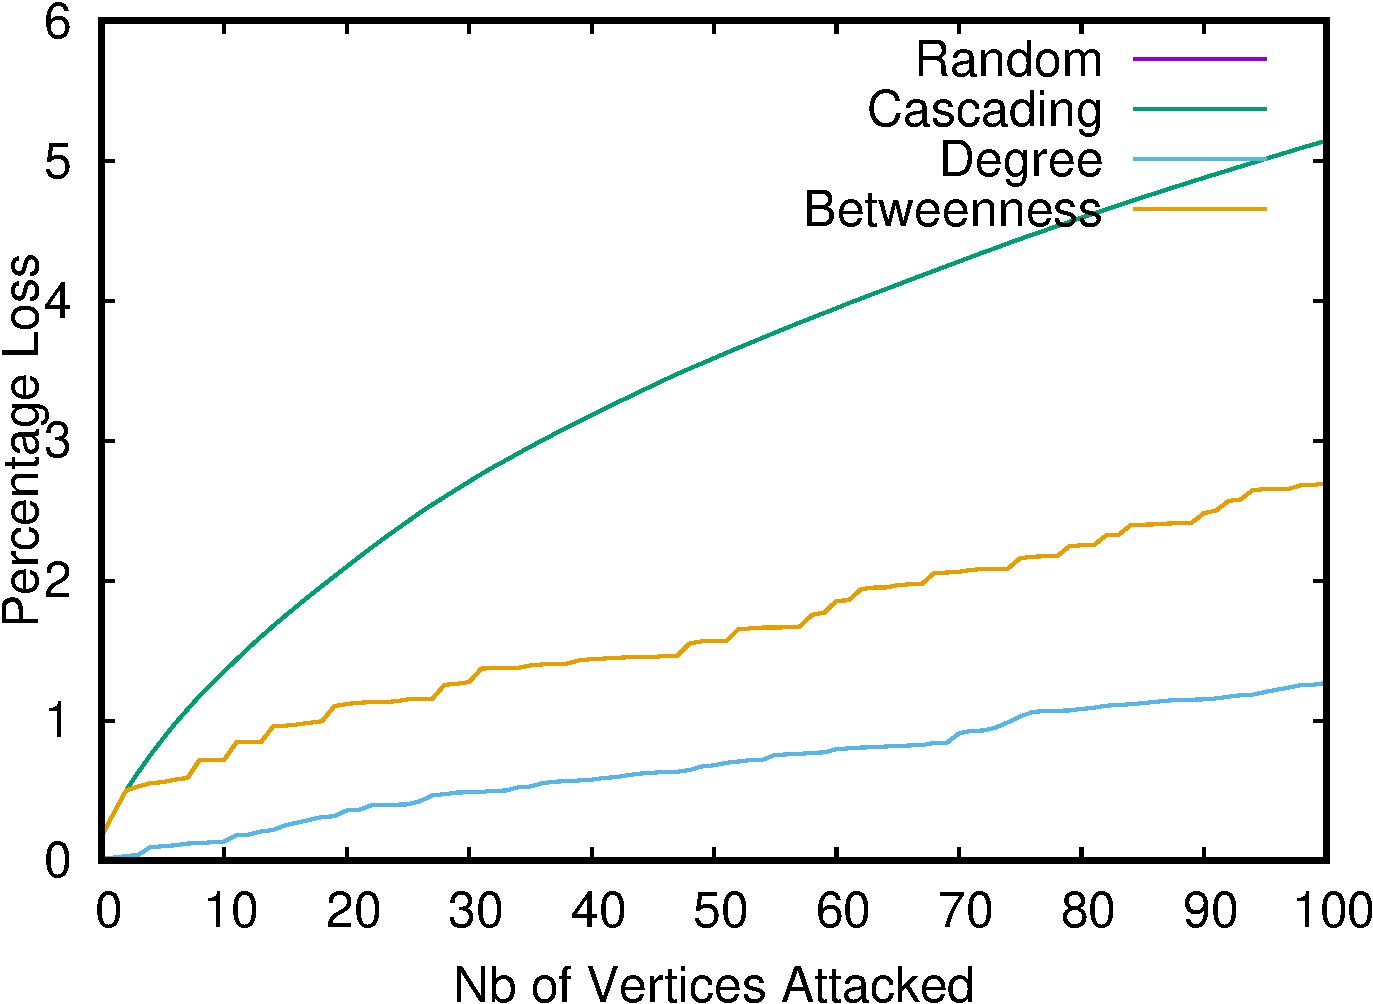
\includegraphics[scale=0.35]{bench/generated/loss-100-crop.pdf}
\caption{Loss percentage: first 100 attacks}
\label{fig:loss-100}
\end{figure}

\begin{figure}
\centering
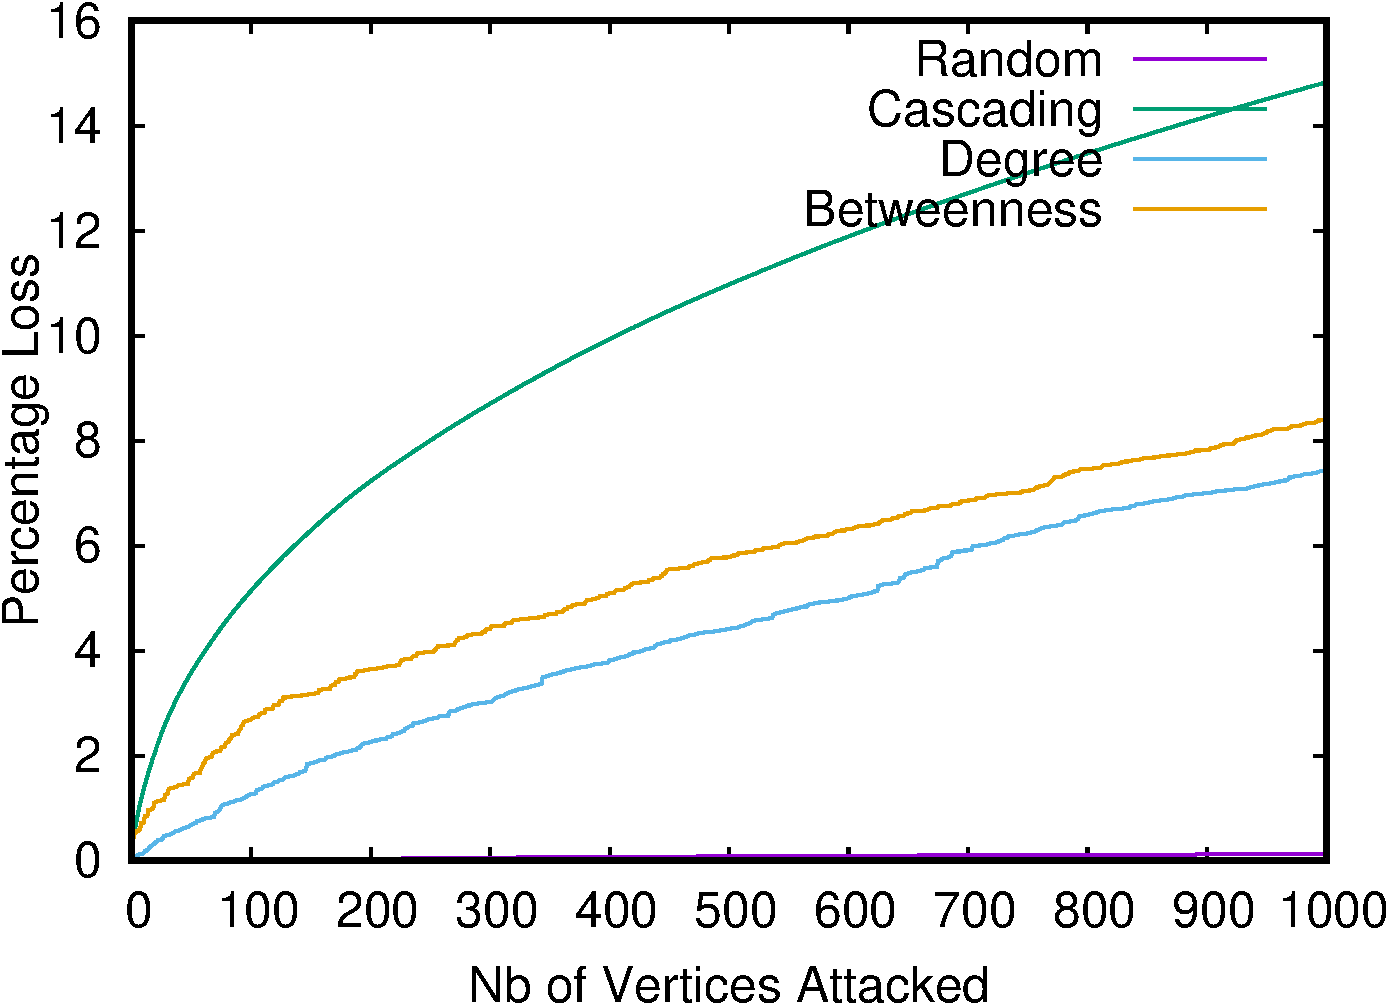
\includegraphics[scale=0.35]{bench/generated/loss-1000-crop.pdf}
\caption{Loss percentage: first 1000 attacks}
\label{fig:loss-1000}
\end{figure}

\begin{figure}
\centering
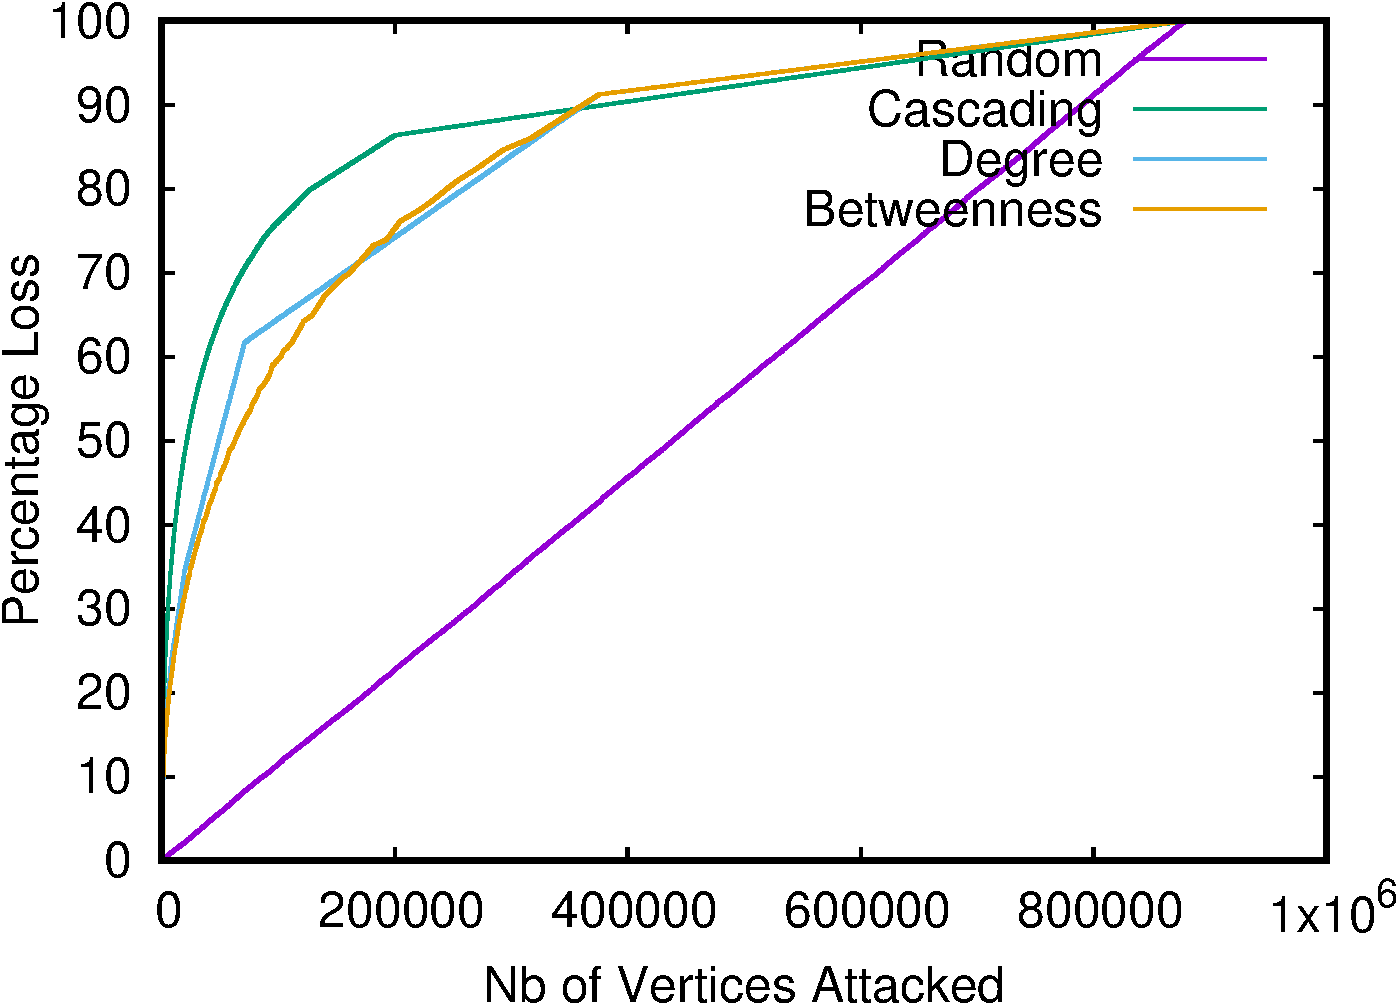
\includegraphics[scale=0.35]{bench/generated/loss-all-crop.pdf}
\caption{Loss percentage: overall attacks}
\label{fig:loss-all}
\end{figure}

\subsection{Run-time and parallel efficiency analysis}
\secondedited{
The run-time for each pair of ({\it thread},{\it partition}) values using our input graphs are shown in the tables~\ref{tab:graph1}, \ref{tab:graph2}, and \ref{tab:graph4}, for $G$, $G_2$, and $G_4$ respectively. Moreover, the corresponding performance efficiency plots are shown in Fig. \ref{fig:effbc1}, \ref{fig:effbc2}, \ref{fig:effbc4}, \ref{fig:effc1}, \ref{fig:effc2}, \ref{fig:effc4}, \ref{fig:effd1}, \ref{fig:effd2}, \ref{fig:effd4}, \ref{fig:effr1}, \ref{fig:effr2}, and \ref{fig:effr4}.  
}
%
\edited{
Here, parallel efficiency is defined as $\frac{T_s}{p\cdot T_p}$, where $T_s$ denotes the serial run-time and $T_p$ denotes the parallel run-time given $p$ parallel processes.}
%
\secondedited{
The timings shown in the tables correspond to the parallel phase of the algorithm. The sequential run-time was omitted because it was extremely negligible compared to the parallel part that is of higher order (in contrast to linear running time in steps 7 and 8).
%
By default, Spark sets the partition size at 64 MB. This is too large for our given graph. As a result, we choose to override the default value by specifying the number of partitions at compile time. When this is done, Spark re-adjusts the size of each partition based on their total number as well as on the size of the input graph. The several connected components in each graph get mapped onto all partitions such that the number of vertices in each partition is balanced across all partitions. We experiment with a number of partitions ranging from $4$, $8$, $16$, and $32$ in order to explore the effect that the number of partitions have on run-time and parallel efficiency. From Fig. \ref{fig:vertices-components-all} and \ref{fig:vertices-components-40}, we gather that there would be enough connected components in each partition to engage all threads assigned to the partition. Also, the fact that many connected components have sizes greater than, say, 40, ensures that the distributed work is more or less balanced.}

As expected, for all three graphs, the fastest and yet the worst parallel efficiency correspond to the R (random failures) scenario that does not rely on any centrality measure computation. In contrast, the highest run-times and hence best efficiency are for the C (cascading scenario) that updates the betweenness centrality of all the nodes following each node removal. It is clear that the more work entailed by a certain scenario, the better it will be for the parallel program to compensate for the overheads associated with the partitioning and scheduling operations. Reading across the three tables for the same partition size and same scenario, our tool shows improved scalability as the input size grows. 

For each given graph and for each scenario employed, we notice that the actual run-time has opposing trends that depend on the number of partitions. For all three tables, there is a cut-off value for the number of partitions, before which run-time continues to improve, and after which it starts to deteriorate. For graph $G$, the cut-off number is at $8$, for graph $G_2$ it is somewhere between $8$ and $16$, and for $G_4$, it is at $16$. We justify the improvement in run-time as we move closer to the cut-off threshold as follows. With a higher number of partitions, one would expect that the multiple threads will be spread about, sharing the work but on data that is more split into distinct regions of main memory. As such, we have reduced contention over the shared address space, as well as scheduling costs associated with managing threads on one single partition. We now argue that creating more partitions beyond the cut-off number drastically affects the performance and introduces a huge overhead -- particularly when the number of threads is low. For instance, in Table II, if we consider only one thread of the BC scenario, it takes 161 (resp. 423) seconds in case of 4 (resp. 32) partitions. We attribute this overhead to the shuffling and repartition operations taking place at the end of each stage that assigns one or more threads from one partition to another. In that phase, some transformations (e.g., \texttt{groupByKey}, \texttt{reduceByKey}, \texttt{join} operations) require shuffling and repartitioning of data, for instance, to group all the items with the same keys in the same partition. 

With that said, we observe that efficiency actually improves for larger partitions. This isn't to be construed, however, to mean that the parallelisation has improved in any way, but rather that the rate of deterioration in the performance for a smaller number of threads (particularly, the case of one thread) is higher when the number of partitions exceeds the cut-off number, resulting in a higher-speedup as the number of threads grows larger. 

%Our own Spark implementation of contingency analysis executes in real-time for the entire power grid, achieving a speed-up of ? on ? processors. We conclude with a spatial understanding of the hotspots on Lebanese soil where energy centers can be exposed and are at risk, using a spatial correlation supported by a binary search tree. The amenability of our work to big data processing makes it extendable to larger networks of networks, towards a fuller understanding of resilence at many vital levels beyond the power grid. Examples are as communications network, Internet networks, transportation networks, hospitals and medical centers networks, to name a few.

\secondedited{
Moreover, we notice that the parallel efficiency in some cases is above one (e.g., in case of betweenness centrality 32 partitions and 2 threads). This may due to the effect of the garbage collectors. In case of one thread and several partitions, the threshold of the garbage collector would be reached ahead of time. Whereas in case of more threads/processes, less data needs to be freed.
%
Additionally, another cause behind super-linear speedup can be attributed to the ``caching effect'', which results from the varying speeds in accessing different levels of the memory hierarchy on which the input graph and intermediate data are stored. As the number of threads increases, the data assigned to each thread decreases, rendering it into the smaller cache levels which are faster to access. As a result, the reduction in run-time is not solely explained by the increase in the number of working threads but also in the reduction of the time spent on I/O, which causes the theoretical estimate for parallel speedup to go beyond $p$ (given $p$ threads), or equivalently, for parallel efficiency to go beyond 1.}

%\begin{figure}
%\centering
%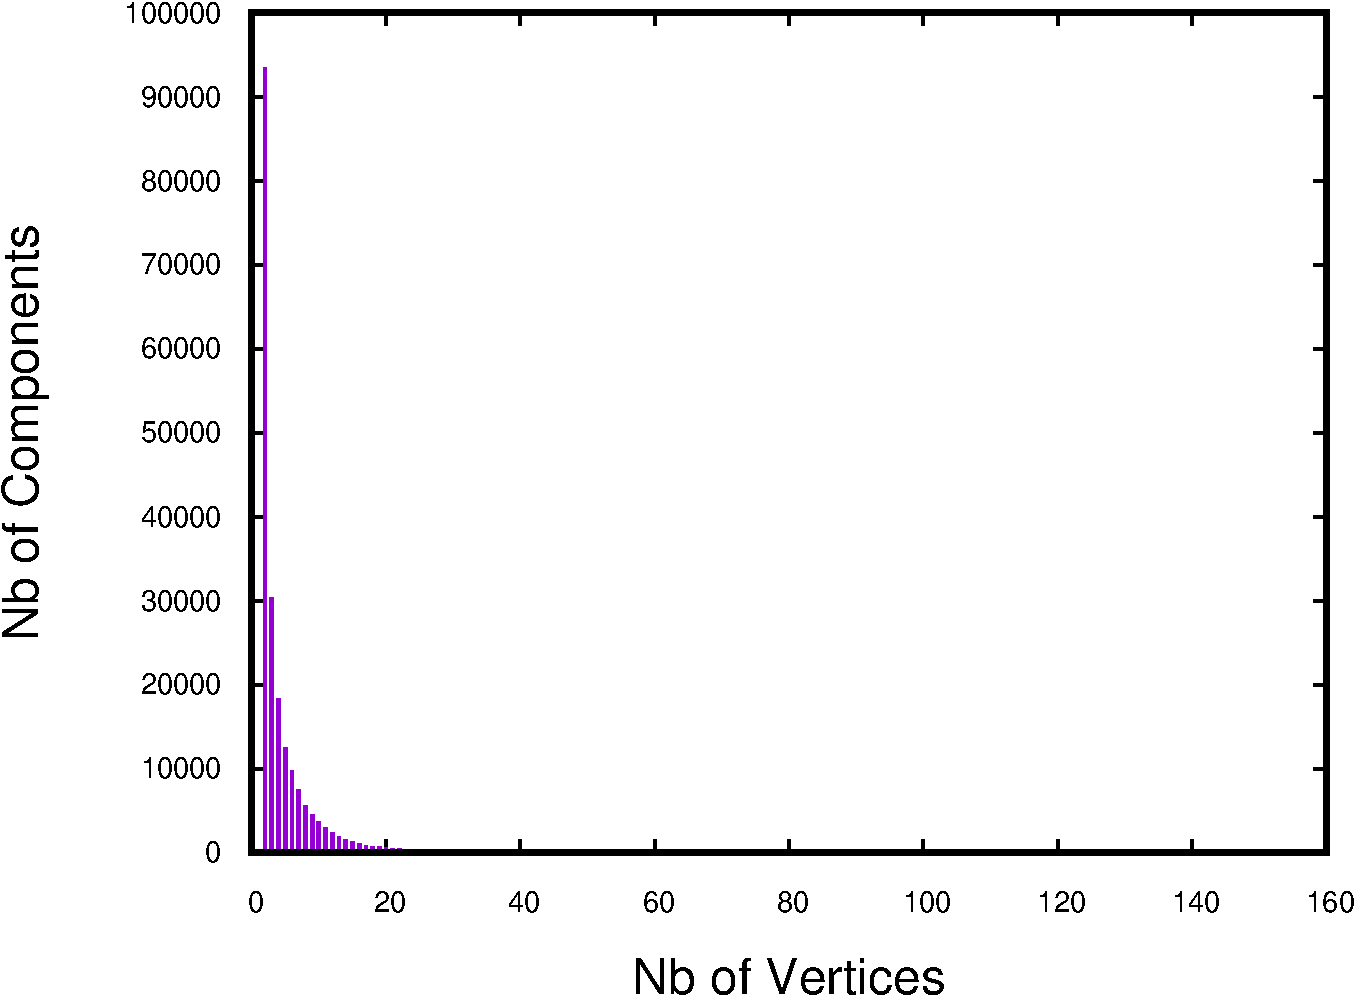
\includegraphics[scale=0.35]{bench/generated/frequencyall-crop.pdf}
%\caption{Components size -- overall distribution}
%\label{fig:cs-overall}
%\end{figure}

%\begin{figure}
%\centering
%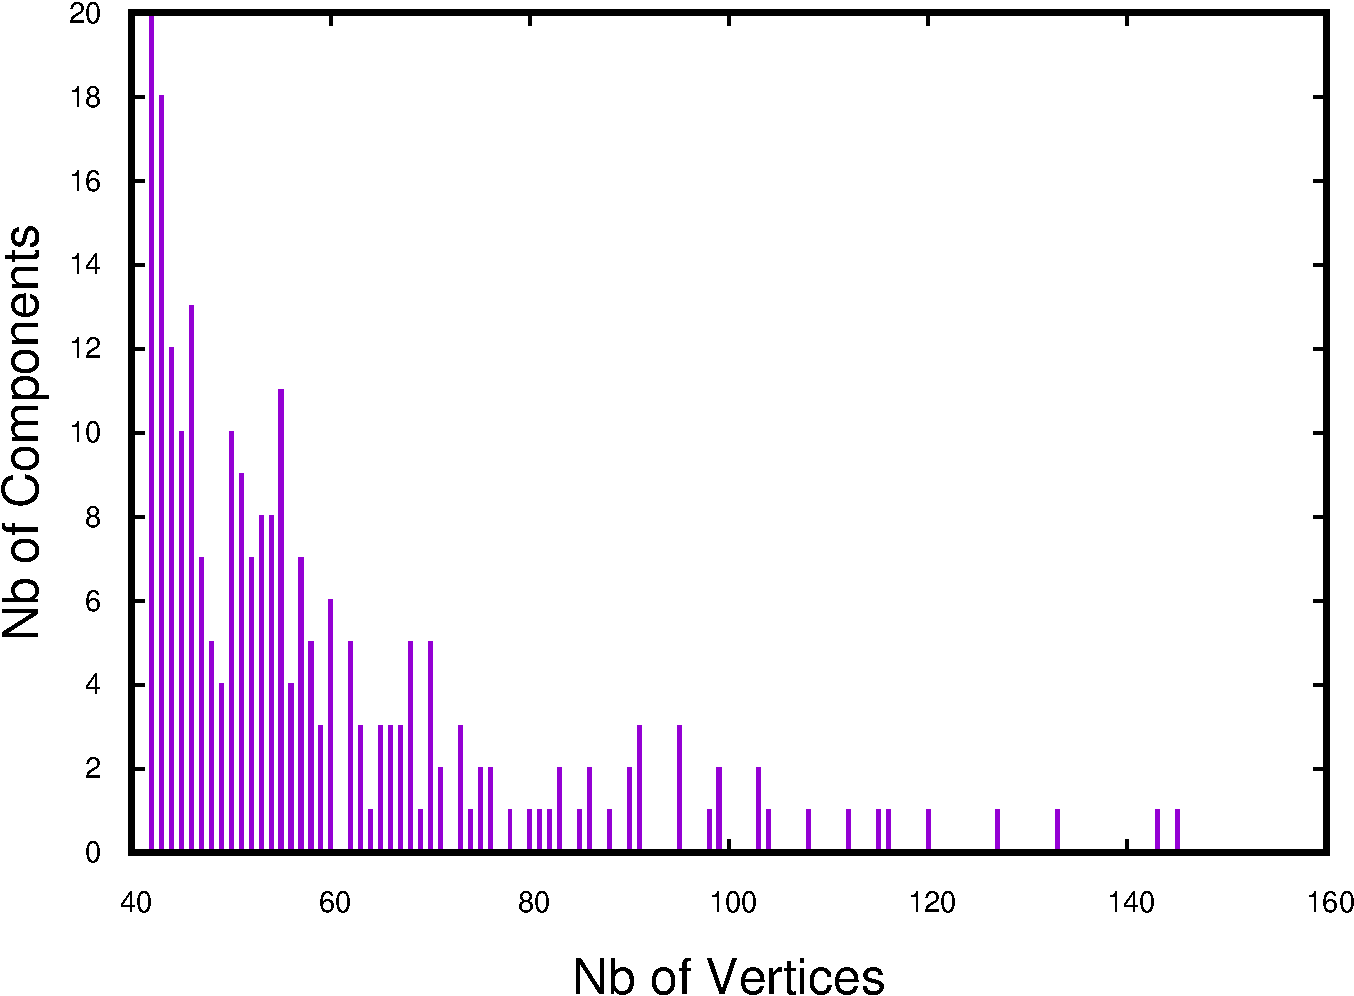
\includegraphics[scale=0.35]{bench/generated/frequency-selected-crop.pdf}
%\caption{Components size -- cropped distribution}
%\label{fig:cs-selected}
%\end{figure}

\begin{table*}[t]
\begin{minipage}[b]{\textwidth}
\caption{Run-time \edited{(in seconds)} for graph $G$}
\label{tab:graph1}
{\small
\centering
\begin{tabular}{||c||c|c|c|c||c|c|c|c||c|c|c|c||c|c|c|c|}
\hline
\textbf{Threads}	&\cellcolor{black!10}BC-4&	\cellcolor{black!10}BC-8	&\cellcolor{black!10}BC-16	&\cellcolor{black!10}BC-32&	\cellcolor{black!10}C-4	&\cellcolor{black!10}C-8&	\cellcolor{black!10}C-16&	\cellcolor{black!10}C-32&	\cellcolor{black!10}D-4&	\cellcolor{black!10}D-8	&\cellcolor{black!10}D-16&\cellcolor{black!10}	D-32&	\cellcolor{black!10}R-4	&\cellcolor{black!10}R-8&	\cellcolor{black!10}R-16&	\cellcolor{black!10}R-32 \\ \hline \hline
64&		27	&17	&22	&41	&53	&34	&32	&52	&26	&15	&20	&41	&23	&17	&20	&39			\\ \hline					
32&		24	&17	&19	&37	&52	&33	&31	&49	&20	&16	&18	&36	&20	&19	&19	&36	\\ \hline
16&		24	&18	&22	&39	&53	&35	&37	&54	&21	&16	&19	&37	&19	&16	&20&37	\\ \hline
8	&	25	&25	&30	&54	&55	&50	&56	&80	&21	&21	&26	&51	&20	&20	&26	&50	\\ \hline
4	&	41	&41	&53	&97	&87	&86	&98	&138	&33	&33	&45	&89	&30	&31	&44	&90	\\ \hline
2&		82	&84	&108	&206	&165	&165	&189	&287	&65	&66	&92	&188	&55	&62	&87	&186	\\ \hline
1&		161	&167	&219	&423	&312	&320	&369	&543	&124	&127	&187	&384	&104	&114	&174	&344	\\ \hline
\end{tabular}
}
\end{minipage}
\end{table*}


\begin{table*}[t]
\begin{minipage}[b]{\textwidth}
\caption{Run-time \edited{(in seconds)} for graph $G_2$}
\label{tab:graph2}
{\small
\begin{tabular}{||c||c|c|c|c||c|c|c|c||c|c|c|c||c|c|c|c|}
\hline
\textbf{Threads}	&\cellcolor{black!10}BC-4&	\cellcolor{black!10}BC-8	&\cellcolor{black!10}BC-16	&\cellcolor{black!10}BC-32&	\cellcolor{black!10}C-4	&\cellcolor{black!10}C-8&	\cellcolor{black!10}C-16&	\cellcolor{black!10}C-32&	\cellcolor{black!10}D-4&	\cellcolor{black!10}D-8	&\cellcolor{black!10}D-16&\cellcolor{black!10}	D-32&	\cellcolor{black!10}R-4	&\cellcolor{black!10}R-8&	\cellcolor{black!10}R-16&	\cellcolor{black!10}R-32 \\ \hline \hline
64		&127	&71	&48	&55	&119	&64	&60	&76	&108	&58	&45	&53	&45	&32	&31	&50		 \\ \hline		
32		&120	&59	&45	&49	&116	&68	&56	&71	&108	&57	&42	&47	&40	&29	&29	&45		 \\ \hline			
16		&128	&66	&39	&52	&115	&66	&65	&79	&112	&57	&36	&50	&41	&33	&30	&46 \\ \hline				
8		&123	&66	&56	&77	&120	&97	&98	&121	&106	&54	&46	&68	&40	&34	&39	&63	 \\ \hline			
4		&164	&104	&101	&142	&210	&191	&185	&223	&134	&83	&80	&119	&60	&57	&69	&113	 \\ \hline			
2		&263	&203	&207	&292	&416	&353	&366	&462	&209	&159	&153	&239	&111	&110	&131	&224	 \\ \hline		
1		&452&357	&371	&525	&761	&804	&793	&969	&355	&281	&286	&434	&196	&201	&230	&402 \\ \hline		
\end{tabular}
}
\end{minipage}
\end{table*}

\begin{table*}[t]
\begin{minipage}[b]{\textwidth}
\caption{Run-time \edited{(in seconds)} for graph $G_4$}
\label{tab:graph4}
{\small
\begin{tabular}{||c||c|c|c|c||c|c|c|c||c|c|c|c||c|c|c|c|}
\hline
\textbf{Threads}	&\cellcolor{black!10}BC-4&	\cellcolor{black!10}BC-8	&\cellcolor{black!10}BC-16	&\cellcolor{black!10}BC-32&	\cellcolor{black!10}C-4	&\cellcolor{black!10}C-8&	\cellcolor{black!10}C-16&	\cellcolor{black!10}C-32&	\cellcolor{black!10}D-4&	\cellcolor{black!10}D-8	&\cellcolor{black!10}D-16&\cellcolor{black!10}	D-32&	\cellcolor{black!10}R-4	&\cellcolor{black!10}R-8&	\cellcolor{black!10}R-16&	\cellcolor{black!10}R-32 \\ \hline \hline
64 &		525&	317	&171&	117	&411	&179&	127	&123	&430	&220	&134	&104&	133&	79&	70	&87	 \\ \hline		
32	&	491&	274	&153	&99	&387	&202	&123	&121 &449	&243&	149&	100	&122	&101&	64&	75\\ \hline
16	&	473	&311	&133	&96	&401	&184	&127	&137 &457	&236	&113	&77	&130	&86	&62	&78 \\ \hline
8	&	557&	250	&132	&126	&387	&234	&204	&212 &452	&222	&113	&105	&119&	93	&75	&93 \\ \hline
4		&750&	333	&221	&234	&612	&431	&374	&398 &601	&274 &168	&190	&151	&126&	120	&163 \\ \hline
2		&1041 &526 &430 &467	&1042	&791	&736	&793 &888	&436	&344	&395	&273	&235	&237	&337 \\ \hline
1		&1626&902&879 &1021 &2156 &1784 &1577 &1754 &1584 &905 &730 &783& 533 &458 &456 &647 \\ \hline
\end{tabular}
}
\end{minipage}
\end{table*}

\begin{figure}
\centering
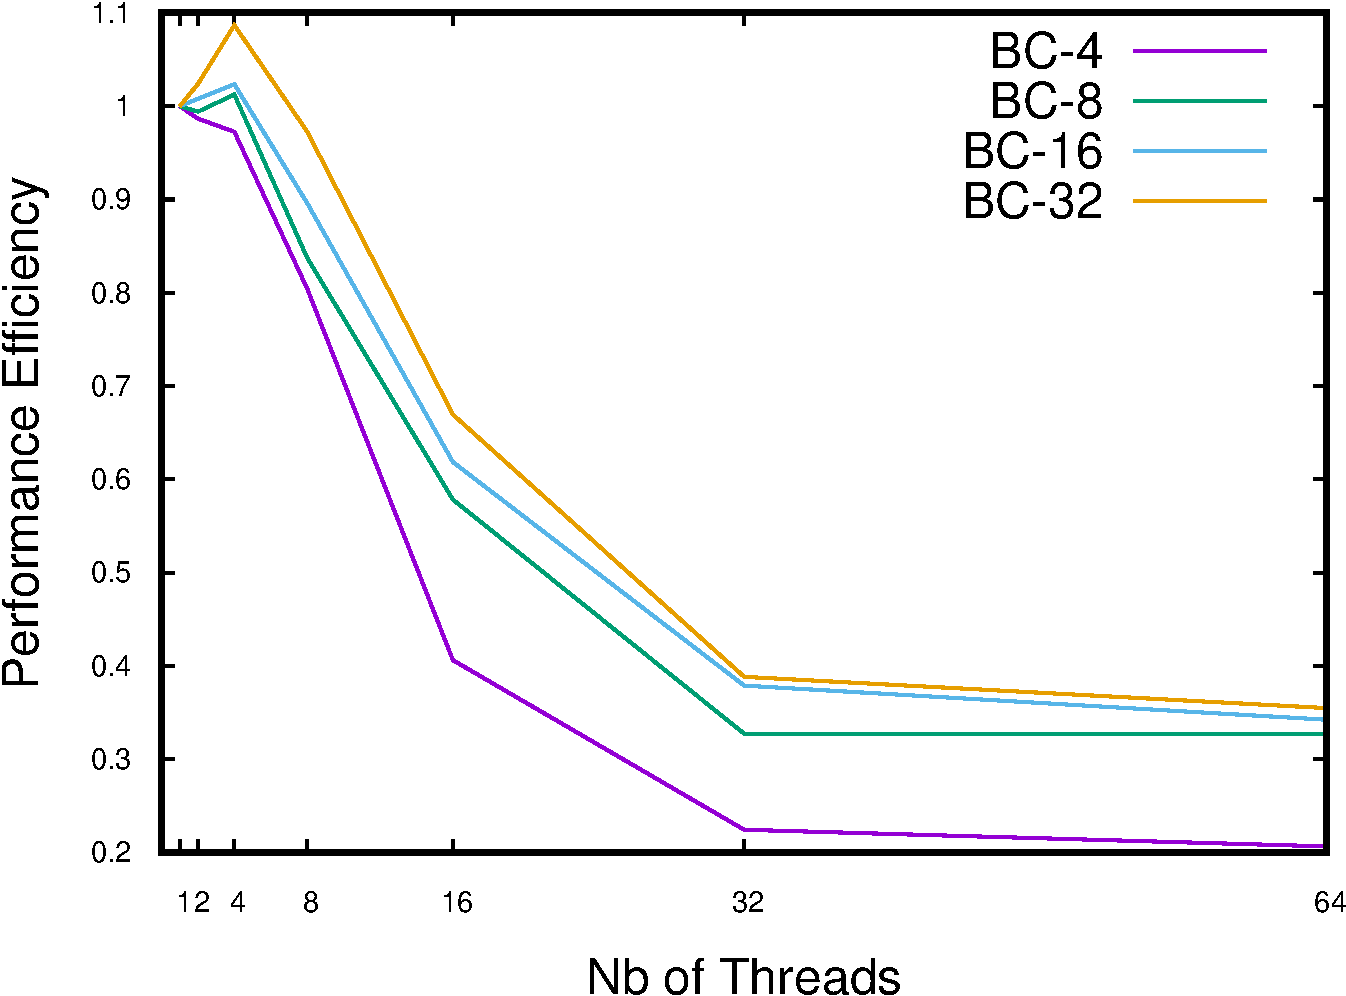
\includegraphics[scale=0.35]{bench/generated/efficiency-bc-1-crop.pdf}
\caption{Efficiency for the load based (BC) scenario and graph $G$}
\label{fig:effbc1}
\end{figure}

\begin{figure}
\centering
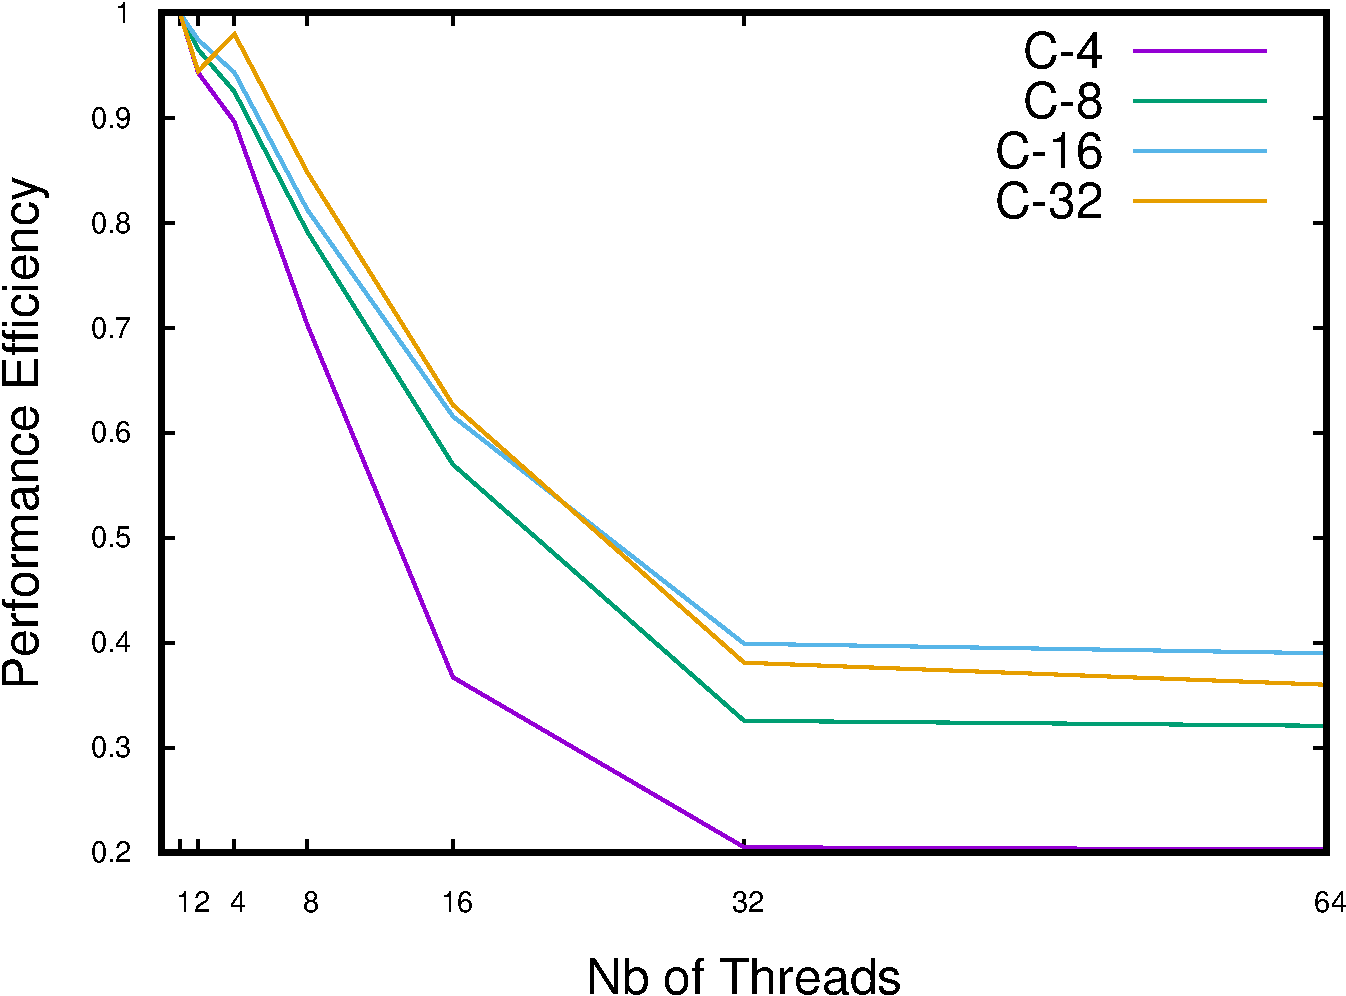
\includegraphics[scale=0.35]{bench/generated/efficiency-c-1-crop.pdf}
\caption{Efficiency for the cascading (C) scenario and graph $G$}
\label{fig:effc1}
\end{figure}

\begin{figure}
\centering
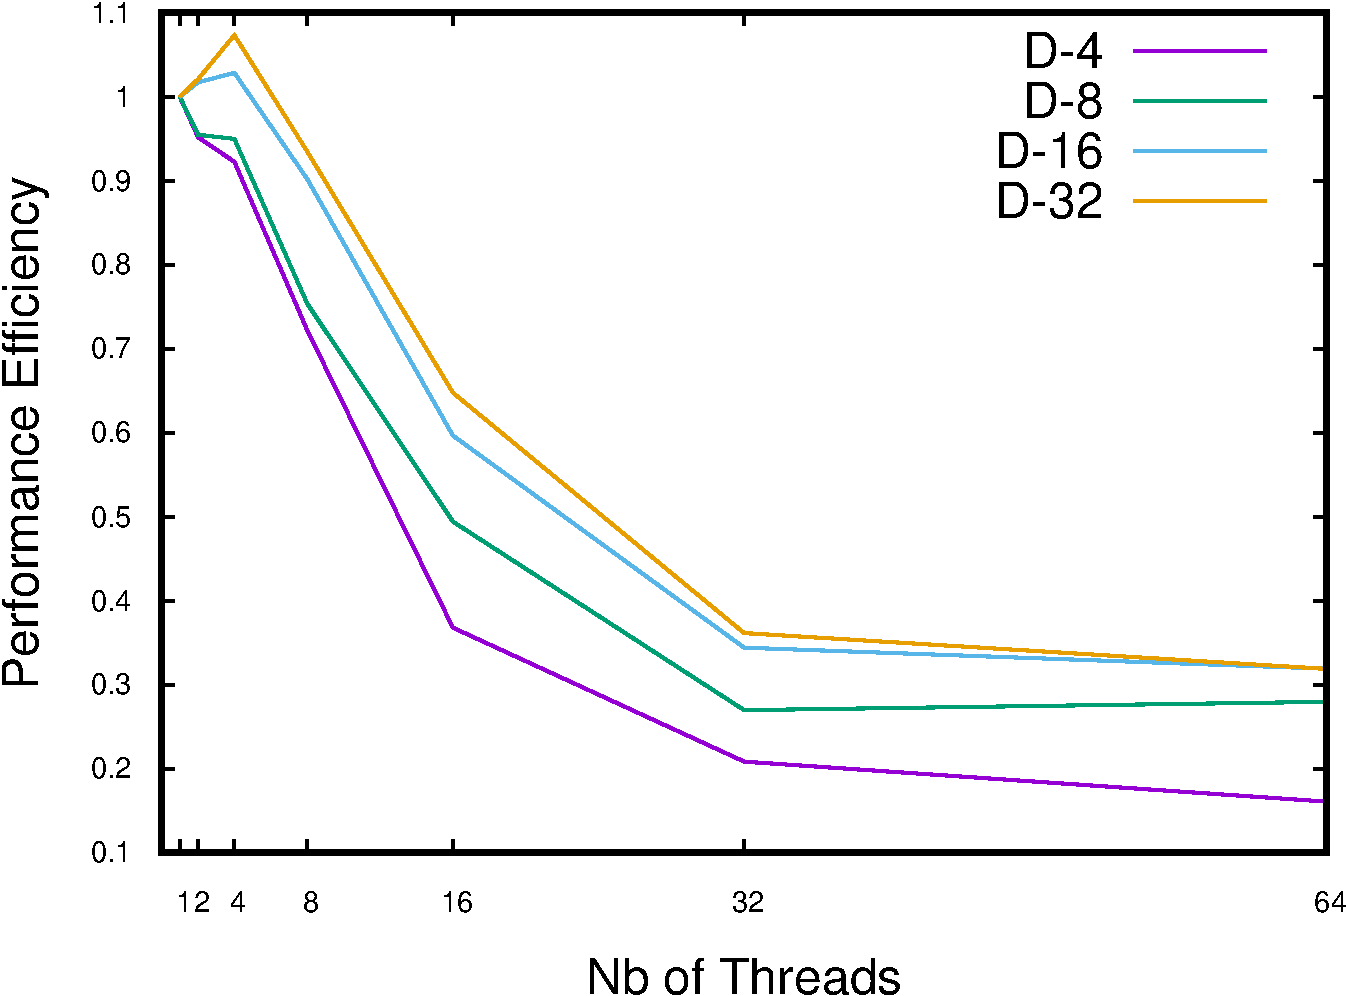
\includegraphics[scale=0.35]{bench/generated/efficiency-d-1-crop.pdf}
\caption{Efficiency for the degree-based (D) scenario and graph $G$}
\label{fig:effd1}
\end{figure}


\begin{figure}
\centering
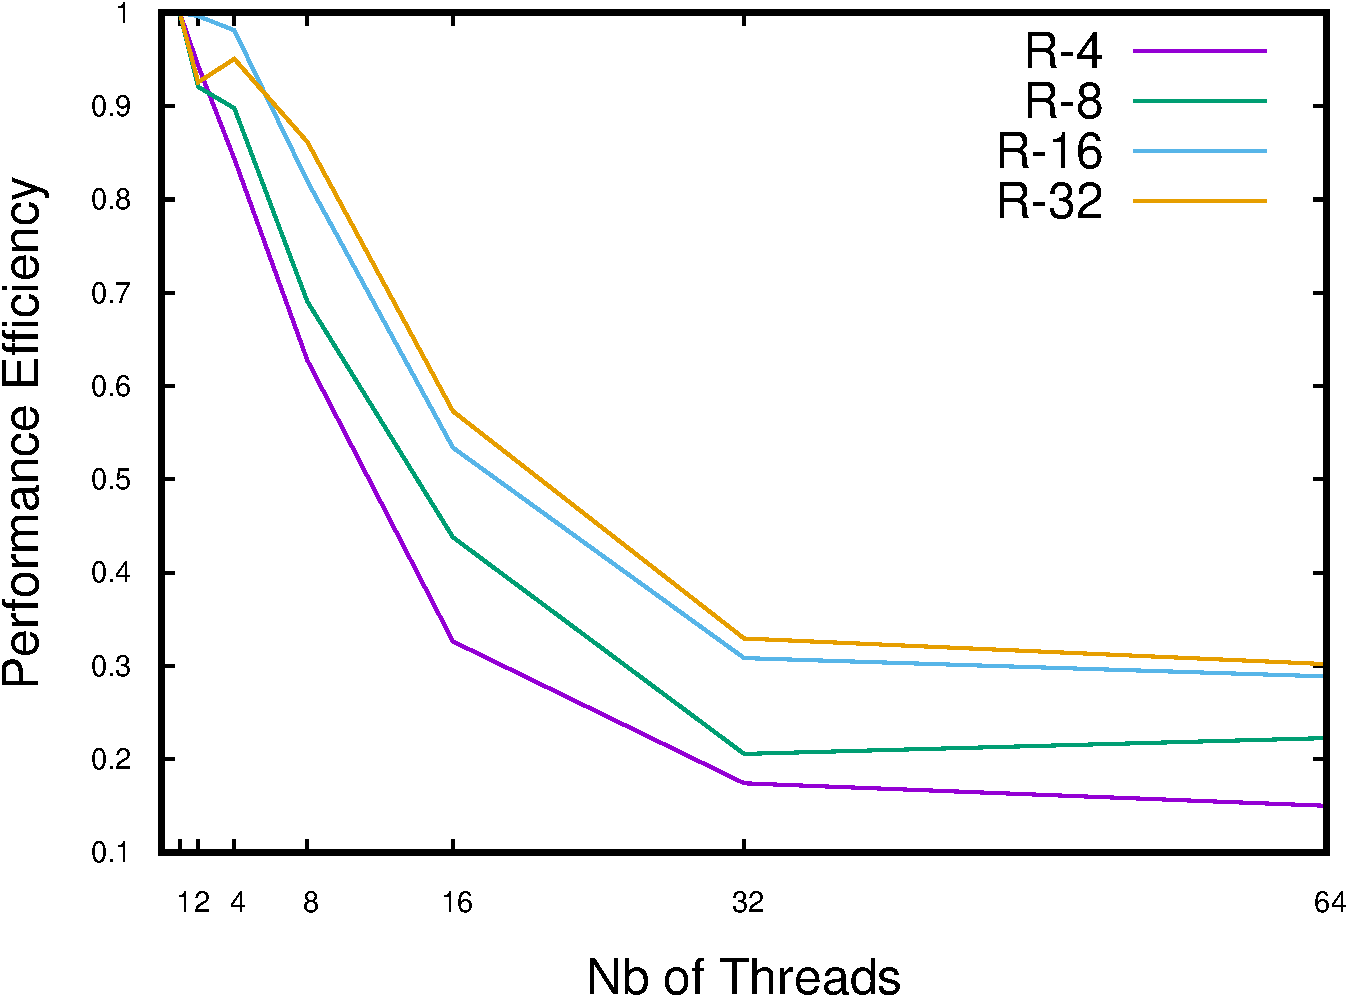
\includegraphics[scale=0.35]{bench/generated/efficiency-r-1-crop.pdf}
\caption{Efficiency for the random (R) scenario and graph $G$}
\label{fig:effr1}
\end{figure}

\begin{figure}
\centering
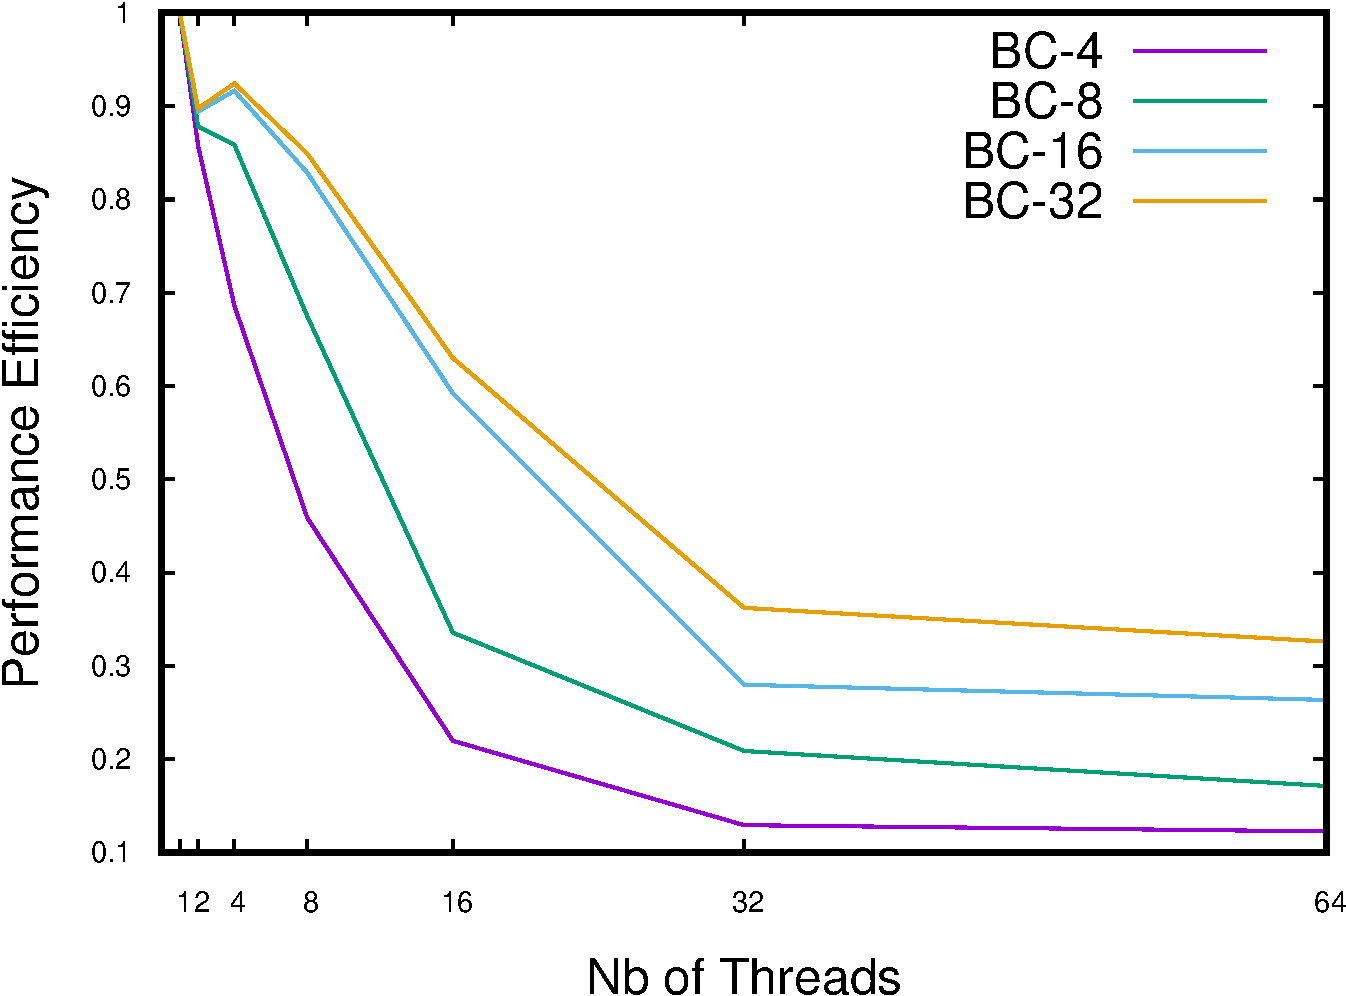
\includegraphics[scale=0.35]{bench/generated/efficiency-bc-2-crop.pdf}
\caption{Efficiency for the load based (BC) scenario and graph $G_2$}
\label{fig:effbc2}
\end{figure}

\begin{figure}
\centering
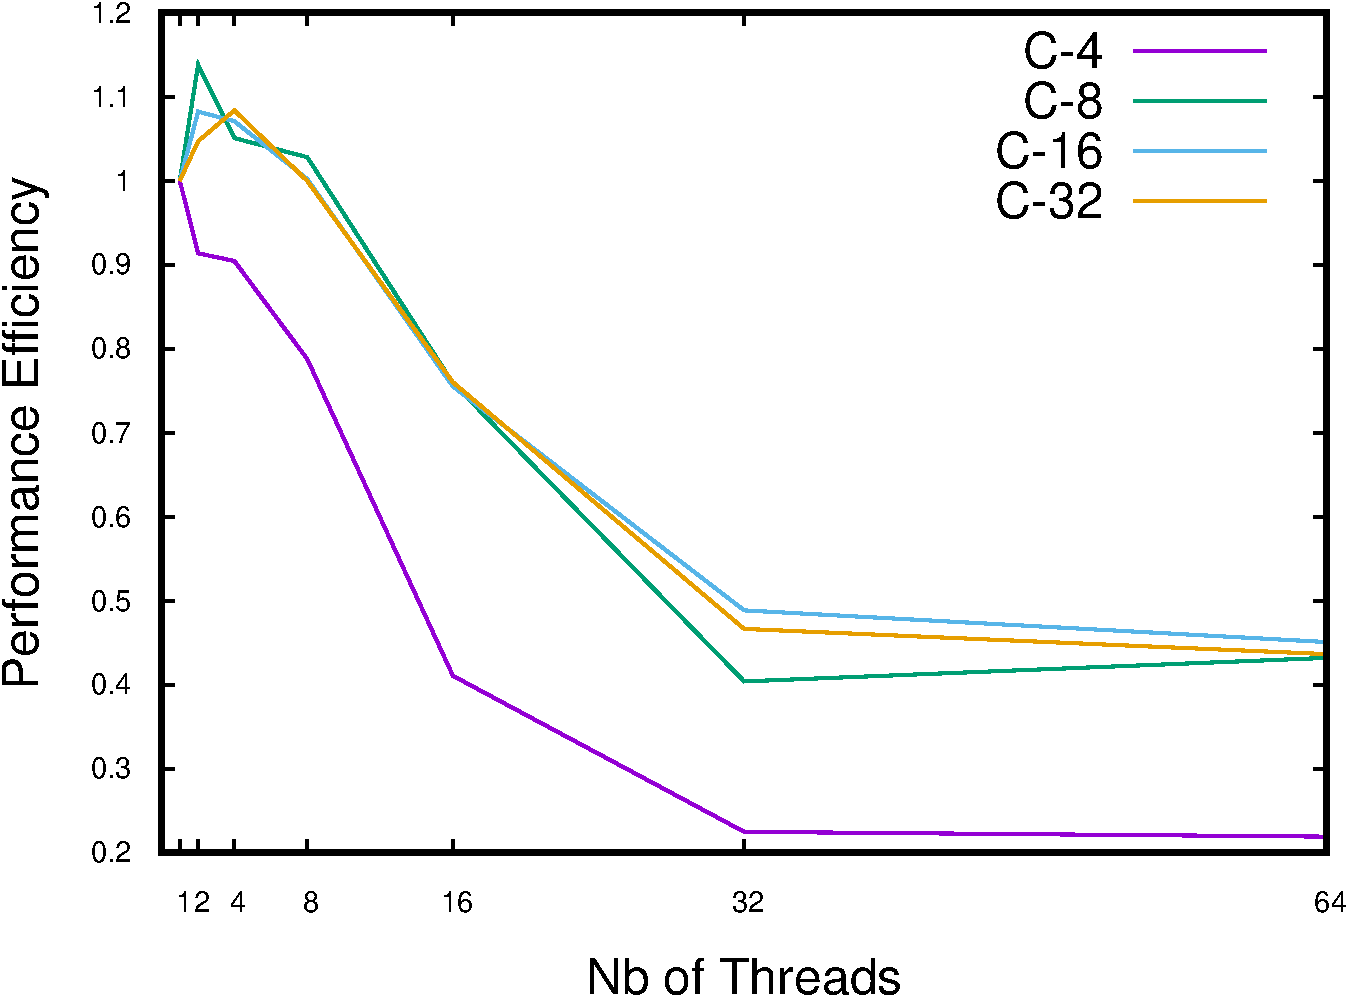
\includegraphics[scale=0.35]{bench/generated/efficiency-c-2-crop.pdf}
\caption{Efficiency for the cascading (C) scenario and graph $G_2$}
\label{fig:effc2}
\end{figure}

\begin{figure}
\centering
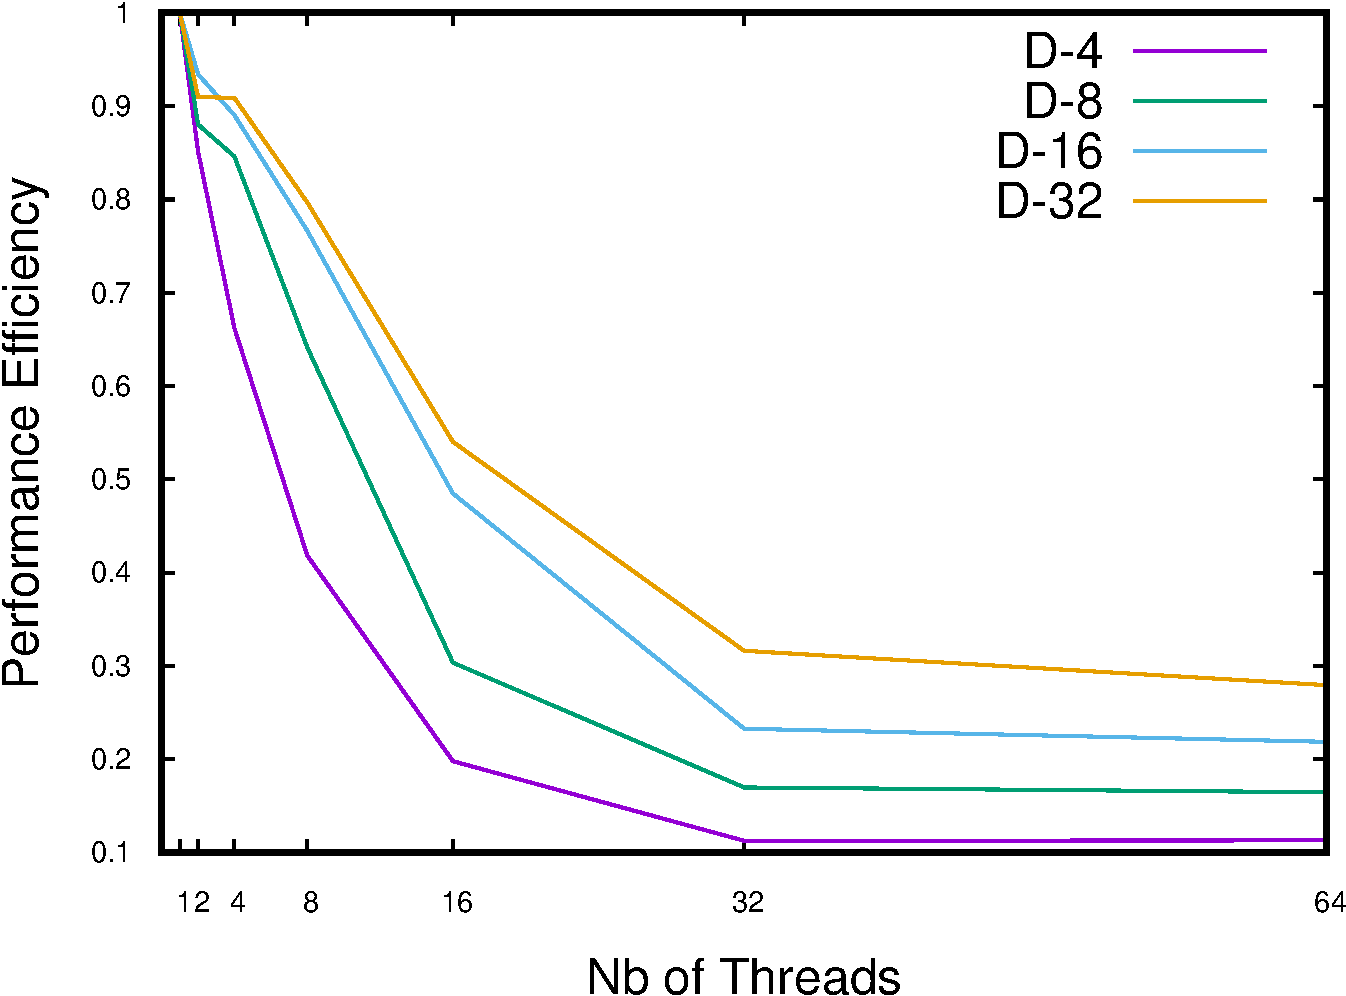
\includegraphics[scale=0.35]{bench/generated/efficiency-d-2-crop.pdf}
\caption{Efficiency for the degree-based (D) scenario and graph $G_2$}
\label{fig:effd2}
\end{figure}


\begin{figure}
\centering
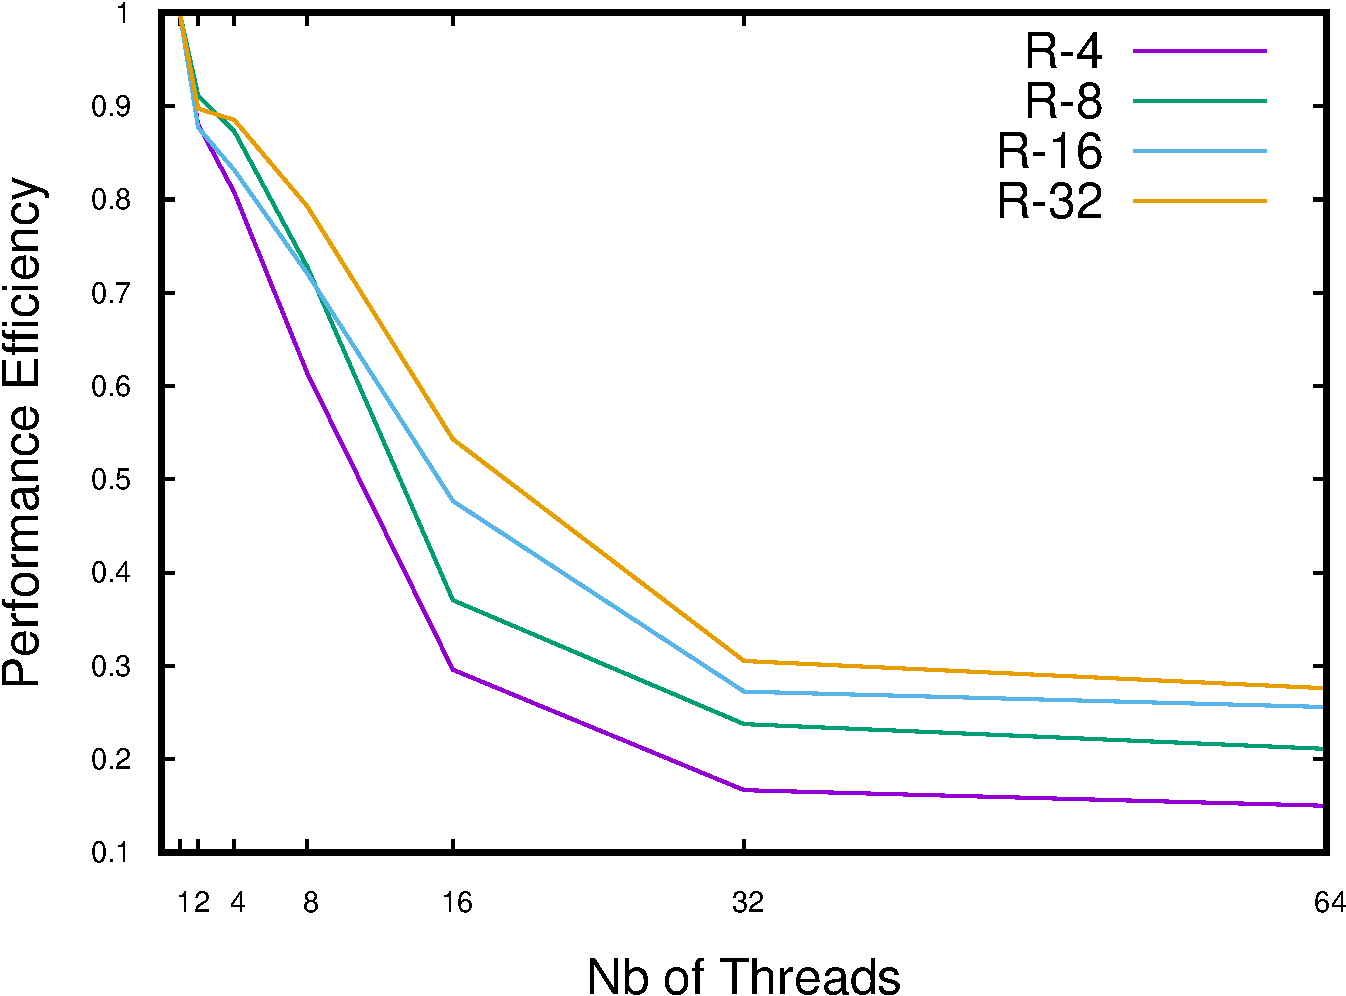
\includegraphics[scale=0.35]{bench/generated/efficiency-r-2-crop.pdf}
\caption{Efficiency for the random (R) scenario and graph $G_2$}
\label{fig:effr2}
\end{figure}

\begin{figure}
\centering
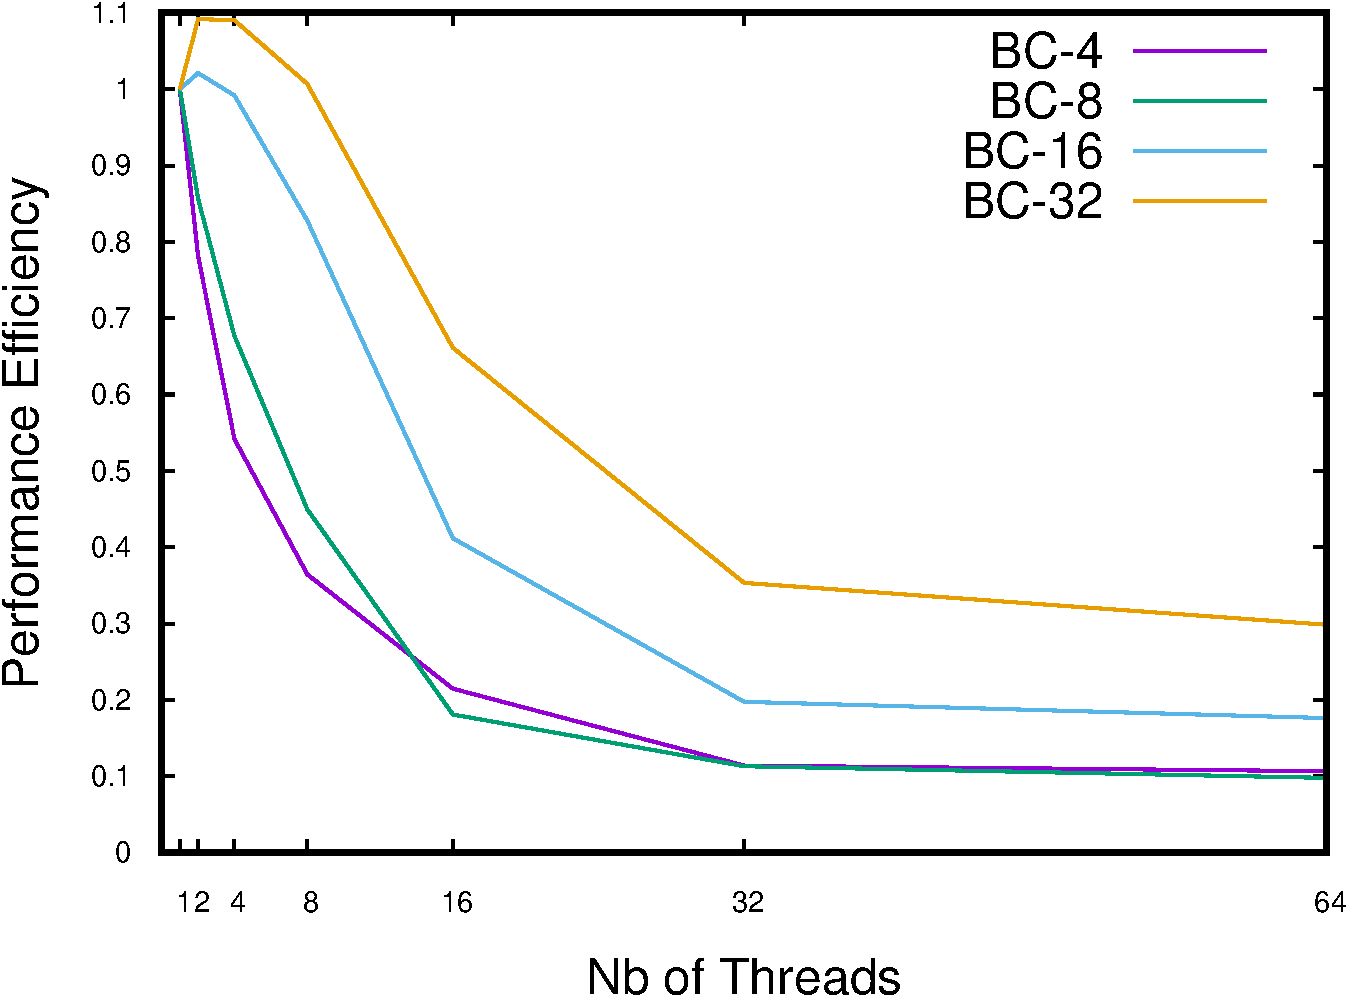
\includegraphics[scale=0.35]{bench/generated/efficiency-bc-4-crop.pdf}
\caption{Efficiency for the load based (BC) scenario and graph $G_4$}
\label{fig:effbc4}
\end{figure}

\begin{figure}
\centering
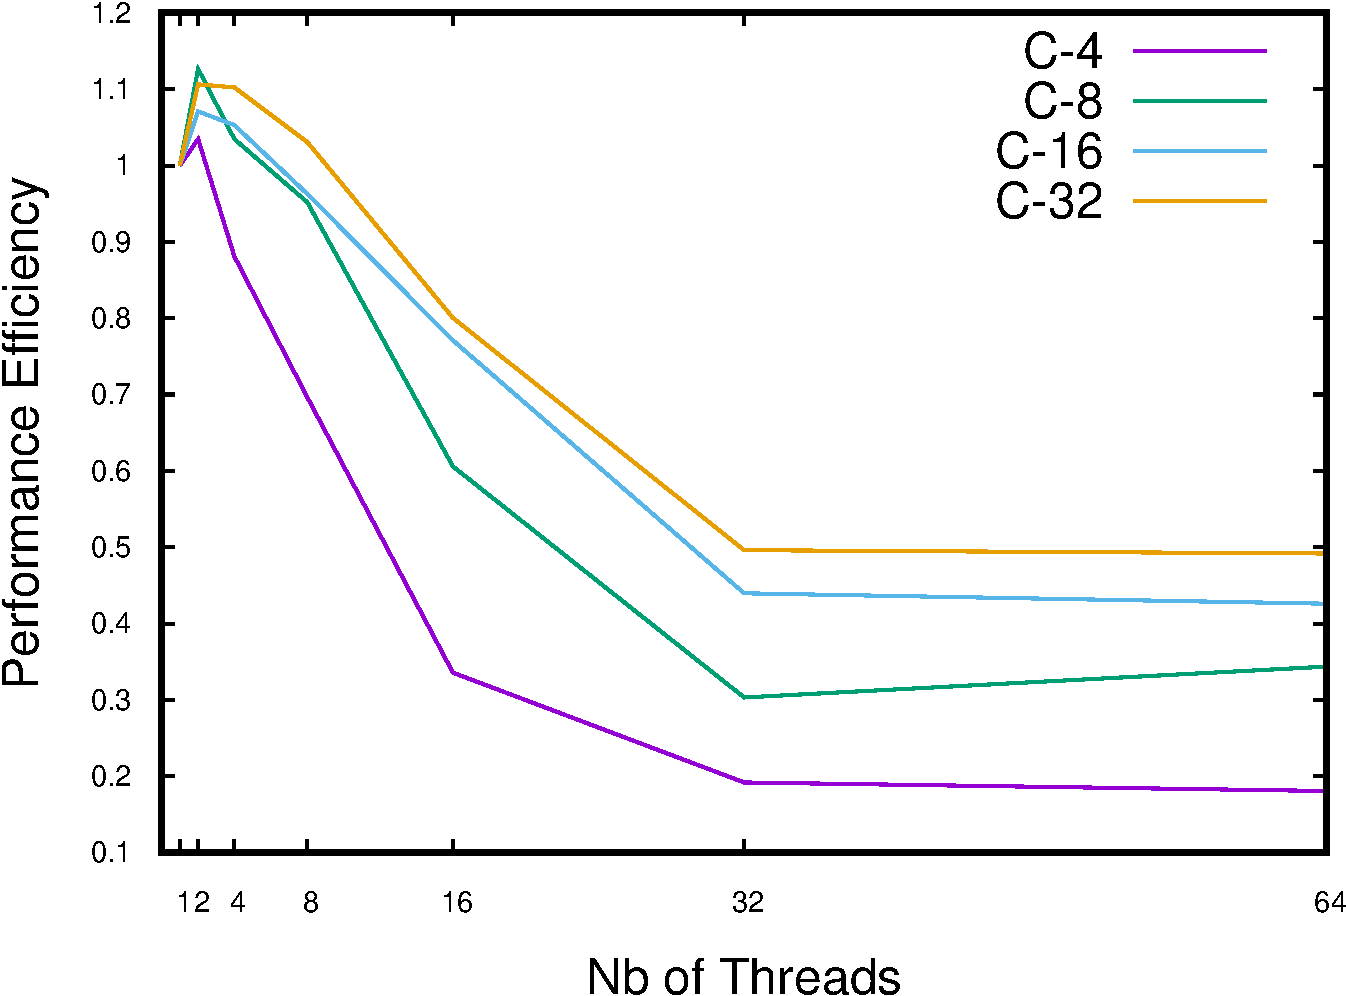
\includegraphics[scale=0.35]{bench/generated/efficiency-c-4-crop.pdf}
\caption{Efficiency for the cascading (C) scenario and graph $G_4$}
\label{fig:effc4}
\end{figure}

\begin{figure}
\centering
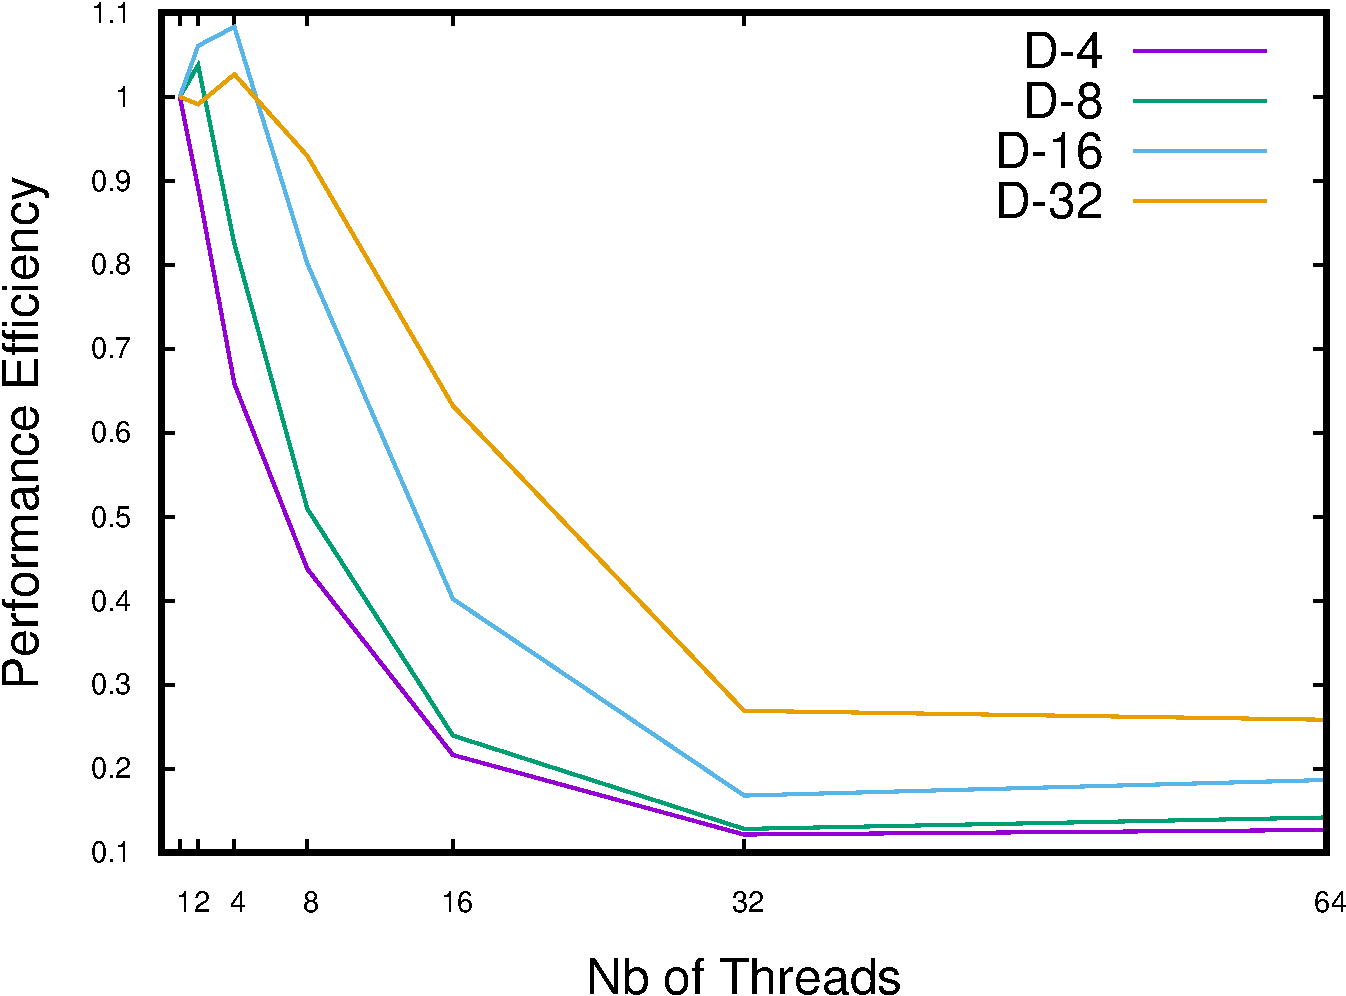
\includegraphics[scale=0.35]{bench/generated/efficiency-d-4-crop.pdf}
\caption{Efficiency for the degree-based (D) scenario and graph $G_4$}
\label{fig:effd4}
\end{figure}


\begin{figure}
\centering
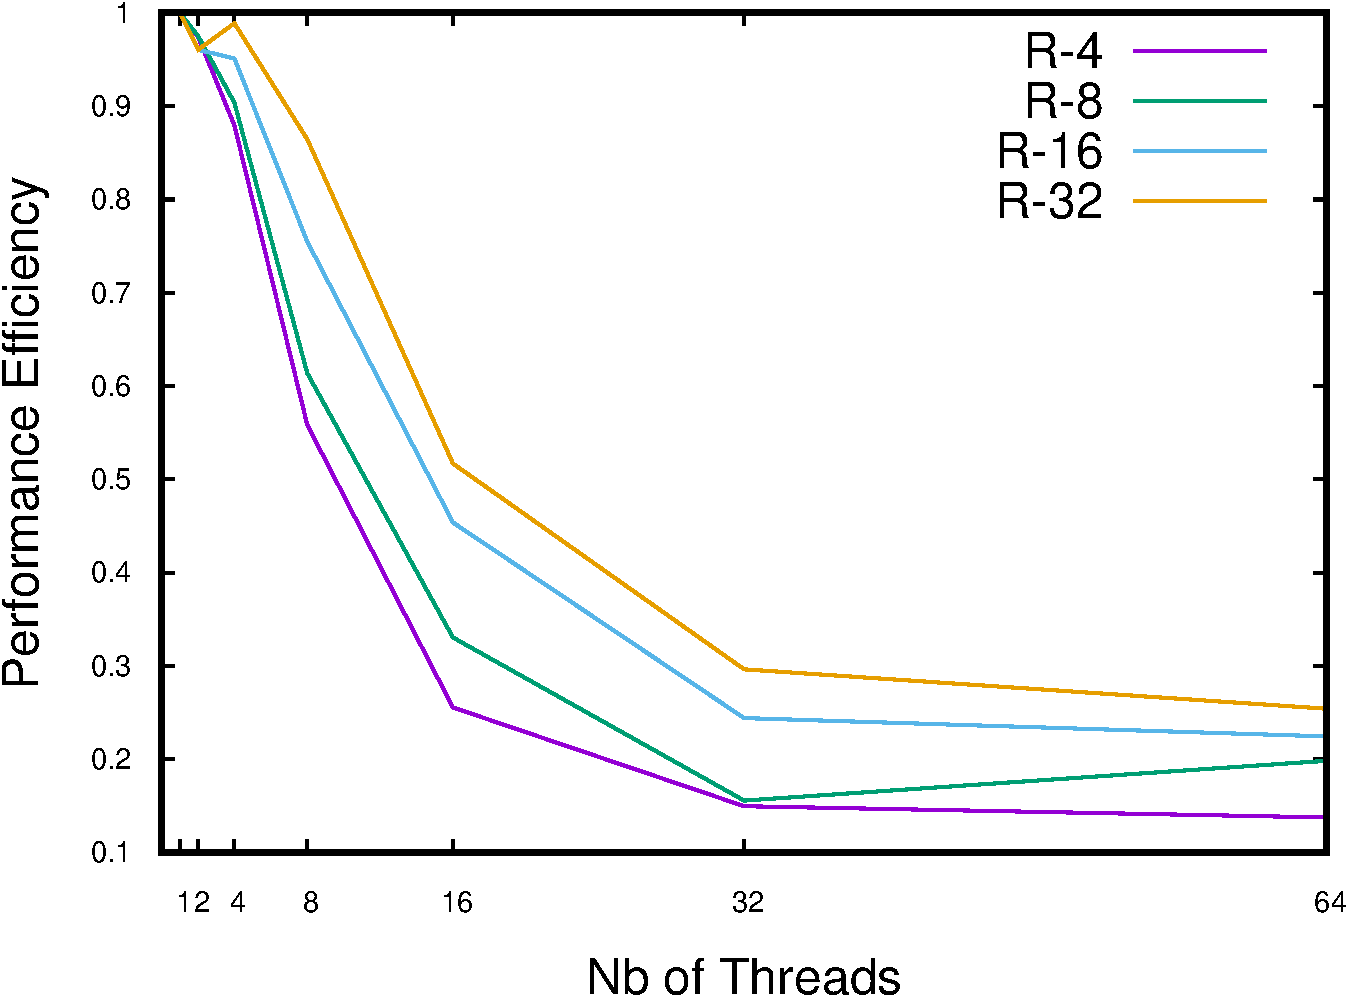
\includegraphics[scale=0.35]{bench/generated/efficiency-r-4-crop.pdf}
\caption{Efficiency for the random (R) scenario and graph $G_4$}
\label{fig:effr4}
\end{figure}



\subsection{Spatial analysis}
The spatial correlation analysis shown in Fig. \ref{fig:correlation} reveals a long range correlated case with correlation decaying slowly with distance, particularly, in the linear regime where $C(r) \propto r^{-\gamma} $, $\gamma = 1.13$, which is in agreement with the literature results in \cite{DaqingAl14}.

\begin{figure}
\centering
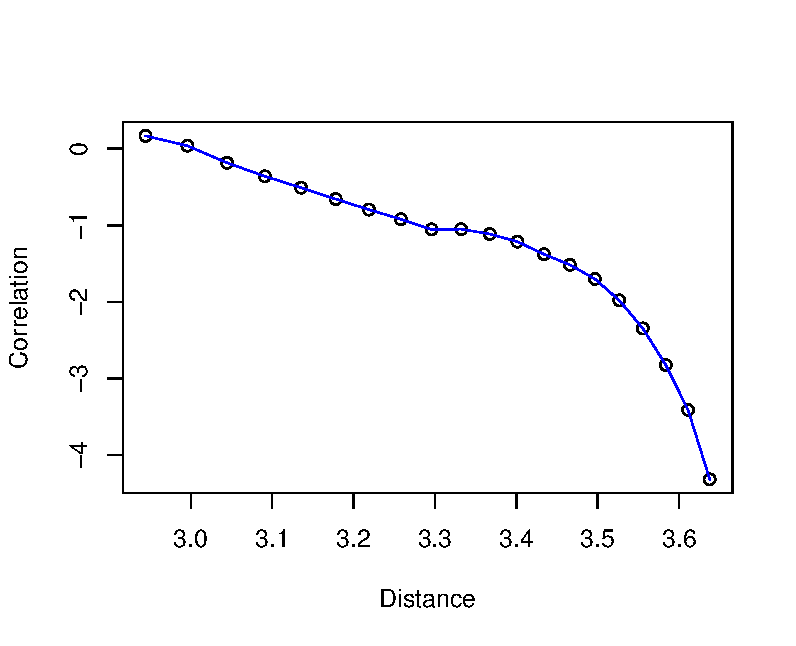
\includegraphics[scale=0.65]{bench/fixed/correlation-eps-converted-to.pdf}
\caption{Spatial correlation between nodes in the cascading scenario on a logarithmic scale.}
\label{fig:correlation}
\end{figure}





\section{Conclusion}
\label{conclusion}
Contingency analysis is a security function to assess the ability of a power grid to sustain various combinations of power grid component failures at energy control centers. To date, there exists no such work to examine the power grid resilience in Lebanon, a country which is still reeling under the effect of a brutal civil war, and recently, bearing an additional burden associated with the spillover from the Syrian war. This neighbouring conflict has exposed Lebanon to a number of random terrorist attacks, and caused it to become one of the major hosts of Syrian refugees, in addition to Iraqi and Palestinian refugees in former years. The strains on Lebanon's vital infrastructure have also been affecting the host community itself, where electric power supply is becoming increasingly drained. Coupled with a severe shortage of funds that can help restructure the entire system, the Lebanese power grid has become plagued with nationwide blackouts, making it an unreliable source of electricity generation, transmission, and distribution. 

\bibliography{biblio}
\bibliographystyle{IEEEtran}


\end{document}


